%!TEX root = ../Demo.tex
\chapter{引言}
\section{研究目的和意义}
视频监控系统是多媒体技术、计算机网络、工业控制和人工智能等技术的综合运用,
它正向着视频/音频的数字化、系统的网络化和管理的智能化方向不断发展\cite{宋磊2003视频监控系统概述}。
视频监控系统是安防领域中的研究热点,随着近年来各类智能设备数量的爆发性增长,
视频监控系统正朝着数字化、智能化、网络化、人性化的方向发展。
它在交通违法抓拍、人脸识别辨别逃犯、停车场车牌识别等安防领域发挥着不容小觑的作用。

近些年来,随着人们生活水平的提高,
% ,监控摄像头不仅仅只出现在公共场所,老百姓的私人空间也会出现监控摄像头的身影。
% 不论在任何国家或地区,
视频监控已经深入每个人的生活,在它的帮助下人们能更好的保护自己和家人的人身以及财产安全。
% 从前,视频监控的唯一作用就是用来监视,记录过去一段时间发生的事情。
% 但是如今视频监控的作用不仅仅局限于此,还提供了例如交通违法抓拍、人脸识别辨别逃犯、
% 停车场车牌识别等等,它在安防领域发挥着不容小觑的作用,
% 对于保障人们日常生产和生活的安全具有重要意义,
% 是大型企业诸如集团化公司、邮电、银行等信息交流广泛的企业生产和管理的必备系统。
% 近些年来,人们生活水平的提高,监控摄像头不仅仅只出现在公共场所,
% 老百姓的私人空间也会出现监控摄像头的身影。
对于安装在公共场所的监控摄像头,其拍摄的视频数据和音频数据都会被相关部门收集并同一管理,
% 其产生的视频数据以及副产物会有相关部门管理,
而这类监控摄像头设备大多是使用电子线缆进行数据传输,会受到时间和地域的双重限制。
% 而且这类监控设备多用电子线缆传送数据,
% 会受到时间和地域的限制;
但是安装在人们家中的监控摄像头就不可能做到由有关部门统一管理,
更不可能在每个用户家中安装一个视频监控的查看终端,
因此就需要一个基于网络的视频监控系统,可以提供在线观看、视频回放等功能。
% 管理就相对分散,需要有个一平台提供,因为不可能在每个用了这类摄像头的老百姓家中塞一个视频监控的查看终端。
基于此,网络摄像头和网络视频监控系统应运而生。

% 以网络为基础的视频监控突破了对时间、地域的限制,只要有网络存在的地方就可以建立网络监控系统,
% 省去了传统的布线和线路维护费用,降低了监控成本;用户在授权的情况下,
% 就可以不受地域时间限制随时按需监控,实现即插、即用、即看\cite{网络视频监控技术的未来发展趋势}。


%视频监控技术的发展,给人们的生活和生产带来了极大的便利和充分的安全保障。
%视频监控系统是安防领域中的研究热点,随着近年来各类智能设备数量的爆发性增长,视频监控系统正朝着数字化、智能化、网络化、人性化的方向发展。
%随着人们生活水平的提高,人们更多的把目光投向了如何更好的保护自己和家人的人身安全以及经济财产,因此以前只出现在公共场所的监控摄像头,如今在人们的家中就能看到它们的身影,希望通过它们可以随时随地的对人或物进行安放监控。

%视频实时监控系统是一个可以实时对远程监控摄像头采集的画面进行实时监测的平台。
%Web端的视频实时监控系统可以依托手机、电脑等支持网页访问的设备进行查看,可以做到只要有网络,就可以随时随地查看监控视频。
%传统的视频监控系统需要在一个局域网内,在一台终端机器上才能实现监控视频的查看。
%本文提出了一种基于Spring Boot的视频实时监控系统的设计思路以及实现方法。


\section{监控系统的发展趋势和研究现状}
\subsection{发展趋势}
上个世纪八十年代,监控系统出现首次出现在人们的生活中,这将近四十年的发展历程可以分为四个主要阶段:模拟监控系统、半数字化监控系统、
全数字化网络监控系统、智能监控系统。

\subsubsection{模拟监控系统}
模拟监控系统是第一代监控系统,主要由三个模块组成:采集模块、传输模块和存储模块。
它们之间的数据交互都是采用的模拟信号,传输介质是同轴电缆。
这一代监控系统往往能支持的监控范围不会很大,因为受到电缆信号传输距离的限制。
此外,因为视频数据是以模拟信号的形式进行传输,存储介质是录像带,这就导致了视频数据的存储、分发和分析极为不便。

\subsubsection{半数字化监控系统}
半数字化监控系统是第二代监控系统,它提供了基“半数字-半模拟”化的监控系统解决方案,所以又被称为“模拟-数字”监控系统。
半数字化监控系统一般由摄像机、数字硬盘录像机(Digital Video Recorder, DVR)、存储设备等组成。
在这一代监控系统中,摄像机通过同轴电缆传输模拟信号给DVR,DVR将模拟信号转化为数据信号,编码压缩后存储,所以同时支持录像和回放。
但是由于仍然使用同轴电缆传输信号,在摄像头数量增加时,布线的复杂程度也会上升。

\subsubsection{全数字化网络监控系统}
全数字化网络监控系统是第三代监控系统,它的诞生意味着监控系统进入了数字化的时代。
第三代系统运用了更为先进的D/A、A/D转换设备视频服务器,
或内置处理器的网络摄像机把图像处理(采集、压缩、协议转换、传输)设置在监控点\cite{百度百科-全数字监控系统},
并通过互联网传输数字形式的视频数据。
这一代监控系统使用的摄像头大多是指出将图像信号编码为数字信号的IP摄像机,因此可以借助强大的互联网传输数据。

\subsubsection{智能监控系统}
智能监控系统是第四代监控系统,它集成了人工智能,可以对图像数据进行分析处理。
得益于人工智能学科的产生和发展,监控系统也朝着智能化的方向发展。
在这一代监控系统中,可以利用计算机对视频和图像数据进行分析,
进而完成以往需要利用肉眼识别的工作,例如人流量计算、车牌识别、违章抓拍等等。
因此,人工智能的出现,极大地扩展了监控系统的适用范围。

\subsection{研究现状}
视频监控支持移动场景。传统的视频监控摄像头大多是固定不动的,可以认为是固定在某一个静止的物体上,
例如房屋的墙上、路灯杆上等等。在这种场景下,可以通过网络布线的方式解决监控中心与被监控点的通信。
但是一旦遇上部署在移动物体上的监控摄像头,例如公交车、高铁等,传统的网络布线方式解决通信问题
显然不可取,还有一种场景就是遇上了复杂地形,高山深谷、河流沙漠等等,同样有限网络也是束手无策。
这个时候支持移动网络的监控摄像头就显得尤为重要,3G、4G、5G等移动网络技术的出现,使得视频监控
支持移动场景变得更加简单。

视频监控支持 IPv6 协议。众所周知,IPv4 的地址已经耗尽,想在公网上继续增加新的 IPv4 地址的网
络监控摄像头有点困难,如果是在局域网中搭建的监控摄像头系统,那么就不会收到这个限制,但是局域网
中的监控摄像头只能在局域网中查看(排除将监控视频上传的公网的情况)。因此需要尽快研发支持 IPv6
v6协议的摄像头。

视频监控支持家庭数字化。数字家庭网络可以由一个的统一的公共网管控制家中的所有智能家居,在视频监控
普及的过程中,不可避免的要和智能家居这个概念联系起来。最终的结果就是视频监控也能支持家庭数字化的
场景,能使用一个统一网关进行操作(观看实时录像、视频回放、抓拍等功能)。

视频监控支持兼容不同设备。
最近几年,监控摄像头的普及非常迅速,现在几乎每家每户都会安装有一个或几个监控摄像头,
这些摄像头可能是同一家公司的产品,也可能不是用一家公司的产品,
% 这其中产生的问题就是兼容性问题,例如摄像头厂商A的摄像头需要在平台A上进行查看,
% 摄像头厂商B的摄像头需要在平台B上进行查看,
而且每个厂商都有自己的协议和平台,这就会产生设备兼容性问题。
% 公司A需要在它自家的平台上才能看到队友监控视频,公司B也是如此。
这就需要制定一个统一个标准,然后所有的厂商按照这个标准去生产摄像头和研发监控摄像头系统。

% 这是因为现在的网络视频监控还没有一个统一个标准,做不到兼容所有的厂家,
% 或者说是每个厂家的生产都没有一个统一标准。

视频监控支持接入人工智能系统。
现在市面上已经存在很多智能的监控摄像头和监控系统,它们具有目标追踪、人物检测等功能。
这些设备的出现,大大减少了人力成本,比如以前要实现摄像头跟踪一个目标,就需要手动去调整摄像头的朝向
但是现在可以使用只能摄像头解决。
% 因此要想转变原本的人力监控,就需要进一步改进当前的视频监控和分析技术,
% 通过视觉技术来分析视频的背景和目标,从而实现目标智能化监控。

\section{本文主要工作}
为了满足视频监控系统数字化、智能化、网络化、人性化发展的需求,
本文基于Spring Boot设计并实现了一个视频实时监控系统。本系统将传统的视频监控系统与网页结合,
拥有链接安防摄像头、查看实时视频、视频保存和查看功能。

系统主要分为服务器端和网页客户端。
服务器端主要使用Spring Boot 编写实现,采用 HTTP 协议与网页客户端交互,接口依照 RESTful 风格编写,
并使用 Java-CV依赖对摄像头视频数据进行采集保存。网页客户端主要使用Vue.js框架编写,主要实现了用户登录、实时监控查看、监控回放查看、增减设备、个人中心、权限管理等功能。
总的来说,本文的主要工作可以概括为以下几点:
\begin{enumerate}
    \item 链接安防摄像头,实时查看视频监控。通过安防摄像头厂商提供的 SDK,代码中引入并调用即可,可以对安防摄像头的视频数据进行读取。
    此外也可以直接使用网络摄像头自带的RTMP或者HTTP-FLV协议格式的视频流地址,实现对摄像头视频的查看和录制。
    \item 视频按时间顺序保存并支持检索。对从安防摄像头上获取的视频数据进行编码,
    保存MP4格式的视频文件到本地磁盘或者分布式存储系统中,以“安防摄像头唯一标识 + 视频时间”作为视频文件的文件名,
    以达到按时间存储的目的,同时在借助数据库保存视频文件的相关信息,支持根据视频文件的开始时间和结束时间为搜索条件进行检索。
    \item 用户登陆和权限管理。不同的用户对监控设备有不一样的可见权限,同时不同的用户对系统的菜单也有不同的可见权限。本文基于RBAC设计了一个权限系统。
    \item 前端页面开发和后端服务开发。前端页面采用 Vue.js框架 进行编写,采用 Element-UI 开源前端组件。后端采用  SpringBoot 框架实现服务,
    % 若后续技术分析中发现服务体量大,会采用 Consul 作为服务发现,用微服务的形式提供。
    采用前后端分离的方式实现,定义RESTful接口交互,实现解耦。
\end{enumerate}


\section{本文结构}
第一章介绍了本课题的研究目的和意义,简述了当前视频监控技术和视频监控系统的研究现状和发展趋势,最后对课题的主要工作进行了概括。

第二章介绍了系统设计过程中涉及到的关键技术。
首先对流媒体传输技术进行了详细介绍,分析比较了RTMP、HTTP-FLV和HLS三个流媒体传输协议。
紧接着对开发框架Spring Boot的功能和特性进行了介绍。
% 、
% MapStruct和数据存储技术Redis

% 最后介绍了RABC权限系统的概念以及设计思路。

第三章从功能性需求和非功能性需求两方面对系统进行了需求分析,然后介绍了系统的数据库设计和系统架构设计。

第四章分别从前端页面和后端服务两个角度对系统关键功能的实现进行了介绍。之后介绍了系统关键功能的测试过程和结果,首先说明了系统的测试环境,然后陈述了系统关键功能的测试用例和结果。


第五章对本文完成的工作进行了总结和归纳,并对监控系统的设计和实现提出了自己的思考。

\chapter{关键技术}
\section{流媒体传输技术}
实时的视频监控系统需要基于流媒体传输技术来实现,需要摄像头本身或者后置的图像处理服务器支持流媒体传输,
常见的三种流媒体传输技术有:RTMP、HTTP-FLV和HLS。

在对这三个协议个优势和劣势进行调研比较之后,决定采用
HTTP-FLV 来实现摄像头实时视频的传输和播放。

\subsection{流媒体以及流式传输}
\subsubsection{流媒体}
流媒体 (Streaming Media) 是在网络上将压缩的多媒体数据流进行传输的技术, 然后用户将压缩包进行解压后就能播放数据流\cite{万梅芬2018基于流媒体技术的数字化校园文化设计与实现}。
它能将一连串的媒体数据(包含音频、视频数据)压缩后并采用流式传输的方式发送。
% ,此技术使得数据包得以像流水一样发送;
如果不使用流媒体,那么就需要在播放音视频等多媒体文件之前下载整个文件。
% 如果不使用此技术,就必须在使用前下载整个媒体文件。
相反的,使用流媒体则不需要下载整个文件,数据会向流水一样依次被客户端加载,一边传输一边播放。
% 流媒体在播放前不会下载整个文件,只将开始部分存入内存,同时也会在用户访问时对数据包进行缓存,让媒体数据正确地输出,
% 流媒体数据流随时传送随时播放。

\subsubsection{流式传输}
流式传输是指客户端通过链接流媒体服务器实时传输音频、视频数据,实现“边下载边播放”。
想要使用流媒体就离不开流式传输。
% 流式传输是实现流媒体的关键技术。
在流式传输中,音视频等多媒体数据通过流媒体服务器向客户端连续地、实时地传输,
所以只需要经过短暂的加载时间,就可以进行观看。
% 流式传输时,音频、视频等时基媒体由音视频服务器向用户计算机的连续、实时传送,
% 用户不必等到整个文件全部下载完毕,而只需经过几秒或十数秒的启动延时即可进行观看。
当音视频等多媒体在客户端上播放时,剩余的部分仍然会由流媒体服务器继续传输。
% 当音频、视频等时基媒体在客户机上播放时,文件的剩余部分将在后台从服务器内继续下载。
流式传输极大的缩短了多媒体文件播放的加载时间。
% 流式不仅使启动延时成十倍、百倍地缩短,而且不需要太大的缓存容量。
% 流式传输避免了用户必须等待整个文件全部从网络上下载才能观看的缺点。

\subsubsection{工作过程}
图 \ref{Fig:server} 展示了流媒体以及流式传输的工作过程。
流媒体数据存储区存放着视频、音频等多媒体数据,这些数据经过发送缓冲区,被编码器编码后发送给客户端。
发送缓冲区和编码器对发送的数据流量进行负反馈调节,防止因为网络拥塞造成卡顿或者数据丢失。
服务端和客户端之间通过流媒体传输协议交互。客户端收到服务端发送的数据之后,进行解码然后在播放器中播放。

\begin{figure}[ht]
    \centering
    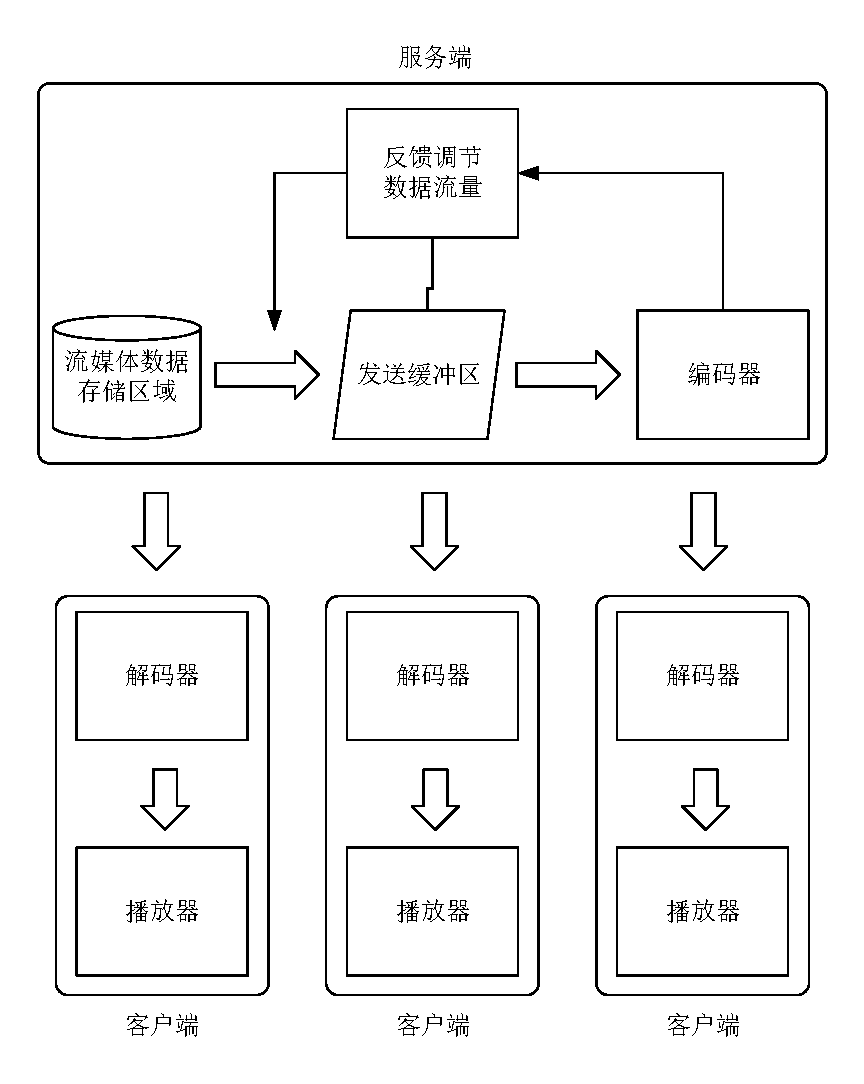
\includegraphics[width=0.8\linewidth]{./Figure/IMG_server.pdf}
    \caption{流式传输示意图}
    \label{Fig:server}
\end{figure}

% 在网络上传输音频、视频等多媒体信息,主要有下载和流式传输两种方案。
% 多媒体文件一般都较大,所以需要的存储容量也较大;
% 同时由于网络带宽的限制,通过下载实现的多媒体数据传输常常要花数分钟甚至数小时,
% 所以这种处理方法延迟也很大。

\subsection{基于RTMP的流媒体传输技术}
% 实时消息传输协议(即Real-Time Messaging Protocol,缩写RTMP) 最初是Macromedia公司为了满足在互联网上传输流媒体音视频而开发的一个私有协议。

% RTMP(Real Time Messaging Protocol) 是由 Adobe 公司基于 Flash Player 播放器对应的音视频 flv 封装格式提出的一种,基于TCP 的数据传输协议。本身具有稳定、兼容性强、高穿透的特点。常被应用于流媒体直播、点播等场景。

% RTMP(Real Time Messaging Protocol) 是由 Adobe 公司基于 Flash Player 播放器对应的音视频 flv 封装格式提出的一种,基于TCP 的数据传输协议。本身具有稳定、兼容性强、高穿透的特点。常被应用于流媒体直播、点播等场景。常用于推推流方(主播)的稳定传输需求

% RTMP,全称 Real Time Messaging Protocol,即实时消息传送协议,
% 最初是Macromedia公司为了满足在互联网上传输流媒体音视频而开发的一个私有协议。
实时消息传输协议(即Real-Time Messaging Protocol,缩写RTMP) 最初是Macromedia公司为了满足在互联网上传输流媒体音视频而开发的一个私有协议。
RTMP是基于TCP的明文协议,端口的缺省值为1935。

RTMP 协议为了维持稳定连续传递,避免单次传输数据量问题,采用了传输层封包,数据流切片的实现形式。
被用来对当前带宽进行划分和复用的最小传输单位,被称为 Chunk 即消息块\cite{流媒体:RTMP协议完全解析}。

一个完整的数据块包含两个部分:Chunk Header 和 Chunk Data,
这两者组合在一起,构成了一个有效的消息类型,结构如图 \ref{Fig:chunk} 所示。
Chunk Header 由基础数据头(Basic Header)、消息数据头(Message Header)和
扩展时间戳(Extended Timestamp)构成。

\begin{figure}[ht]
    \centering
    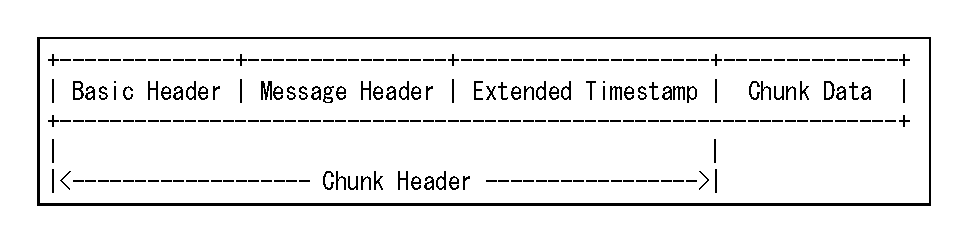
\includegraphics[width=1\linewidth]{./Figure/IMG_chunk.pdf}
    \caption{Chunk 格式示意图}
    \label{Fig:chunk}
\end{figure}

消息(Message)是协议中的基本数据单元,
消息块(Chunk)是比消息更小的数据单元。
在数据发送时,消息会被分割为消息块,然后消息块会通过TCP发送出去。
在数据接收时,消息块会被组装成消息,最终解析成原始的流媒体数据。

通常情况下,一个有效的消息,如果数据量超出 Chunk Size 的话,则会被拆分成多个消息块来分批传输。
默认情况下,Chunk Size 的值为 128字节。

图 \ref{Fig:rtmp} 展示了一则当Chunk Size为128字节是的消息拆分发送过程。
% 协议中的基本数据单元称为消息(Message),传输的过程中消息会被拆分为更小的消息块(Chunk)单元,
% 最后将分割后的消息块通过 TCP 协议传输,接收端再反解接收的消息块恢复成流媒体数据。
一个大小为 500 字节的 RTMP消息,被拆分为4个大小分别为128字节、128字节、
128字节、116字节的消息块,最终通过TCP发送出去。

\begin{figure}[ht]
    \centering
    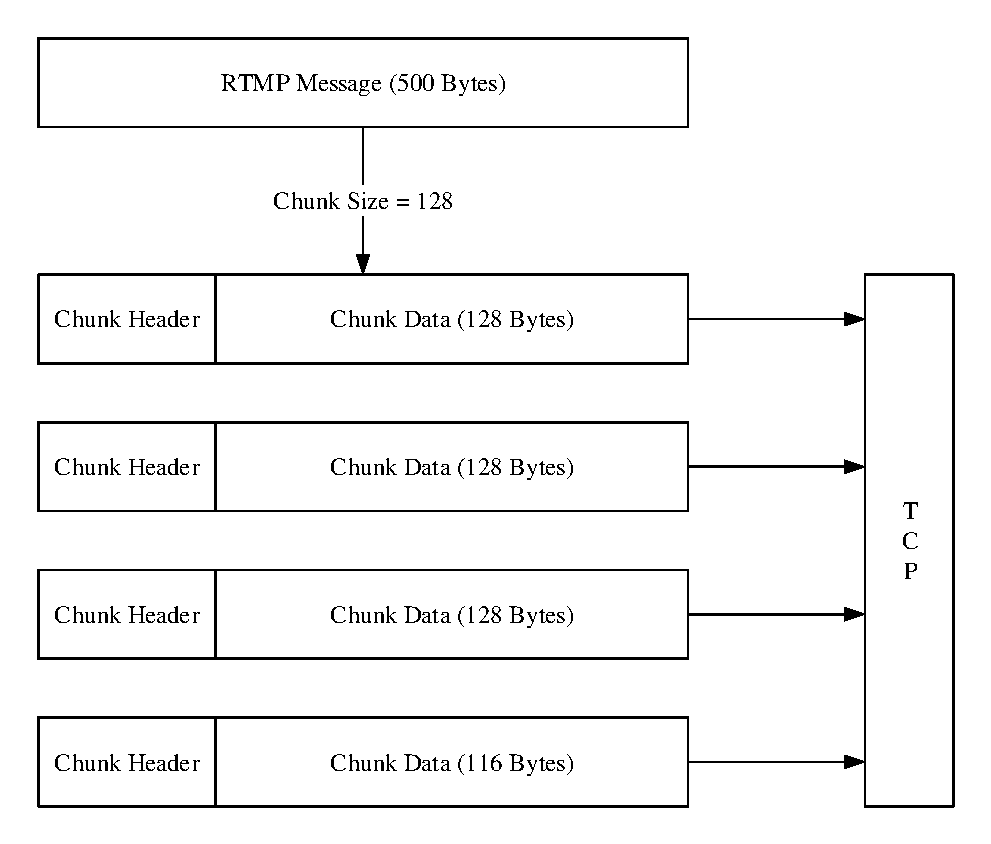
\includegraphics[width=1\linewidth]{./Figure/IMG_rtmp.pdf}
    \caption{消息拆分示意图}
    \label{Fig:rtmp}
\end{figure}

% 通过指定首个 Chunk 和后续 Chunk 类型,以及 Chunk Header 其他标志性数据,来使当前被切割的消息,能够在对端得到有效的还原和执行。我们以 MetaData 类型消息(Data AFM3 16)举例:
% \newpage
% RTMP主要有以下几个优点:
% \begin{enumerate}
%     \item RTMP 是专门为流媒体开发的协议,对底层的优化比其它协议更加优秀。
%     \item 基本上所有的编码器(摄像头之类)都支持 RTMP 输出,。
%     \item RTMP适合长时间播放,并且具有较低的延时,一般延时在 1-3s 之间。
% \end{enumerate}

% RTMP并不是完美的,也有不足之处。
% 一方面是它是基于 TCP 传输,没有像HTTP那样的公共端口,被防火墙拦截的可能性也更大;
% 另一方面是Adobe并没有完全开源RTMP协议,这就导致很多设备无法需要使用第三方解码器才能播放。
\newpage
\subsection{基于HTTP-FLV的流媒体传输技术}
HTTP-FLV协议
首先会将流媒体数据按照FLV格式进行封装,然后再使用HTTP传输封装之后的数据。
% 是将流媒体数据封装成 FLV 格式,然后在通过HTTP协议进行传输。

FLV是一种适用于流式传输的网络视频格式,全称为Flash Video。
% Flash Video(简称FLV),是一种网络视频格式,用作流媒体格式,
% 它的出现有效地解决了视频文件导入Flash后,使导出的SWF文件体积庞大,
% 不能在网络上有效使用等缺点\cite{WIKI_FLV}。
FLV 文件格式由FLV Header 和 FlV Body 组成。
FLV Body 由多个Tag构成,每个Tag 包含 Tag Header 和 Tag Data 组成。
FLV 协议的格式如图 \ref{Fig:flv} 所示。

\begin{figure}[ht]
    \centering
    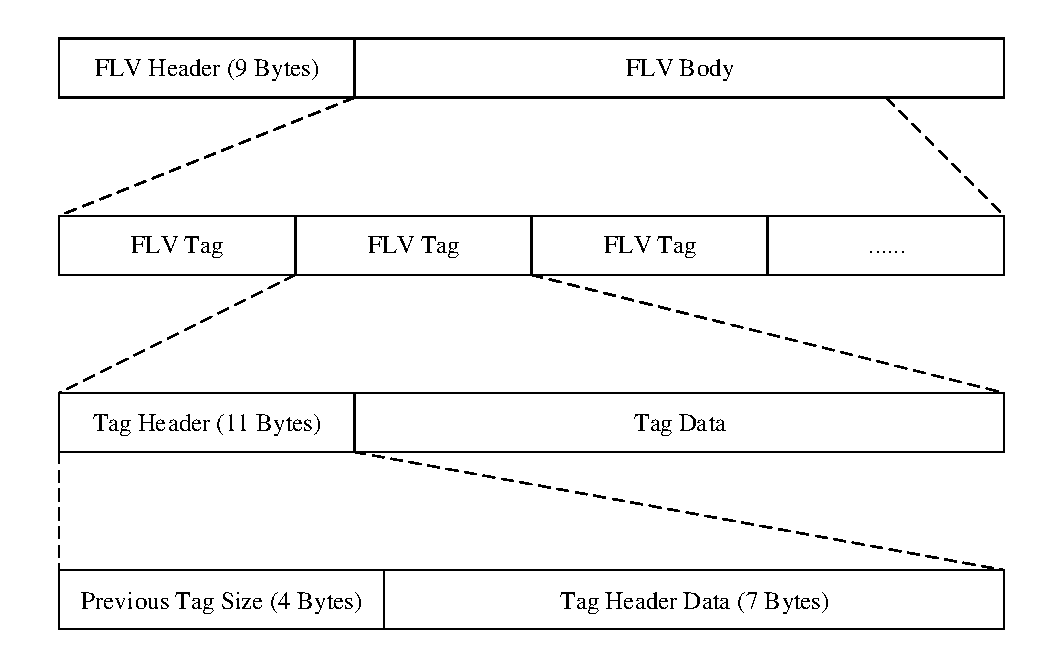
\includegraphics[width=0.8\linewidth]{./Figure/IMG_flv.pdf}
    \caption{FLV协议格式}
    \label{Fig:flv}
\end{figure}

\newpage
FLV Tag 共有三种类型,分别是Video Tag、Audio Tag和Script Tag,
通过 Tag Header Data中的第一个字节来区分。
Video Tag后的Tag Data中存放的是视频相关数据;
Audio Tag后的Tag Data中存放的是音频相关数据;
Script Tag后的Tag Data中存放的是音视频元数据。

FLV Tag 中的前四个字节用来表示前一个Tag 的长度,即图 \ref{Fig:flv} 中的Previous Tag Size字段。
因此,整个 FLV Body 部分可以通过这个字段完全串联起来,形成一个完整的文件,如图 \ref{Fig:flv_file} 所示。

\begin{figure}[ht]
    \centering
    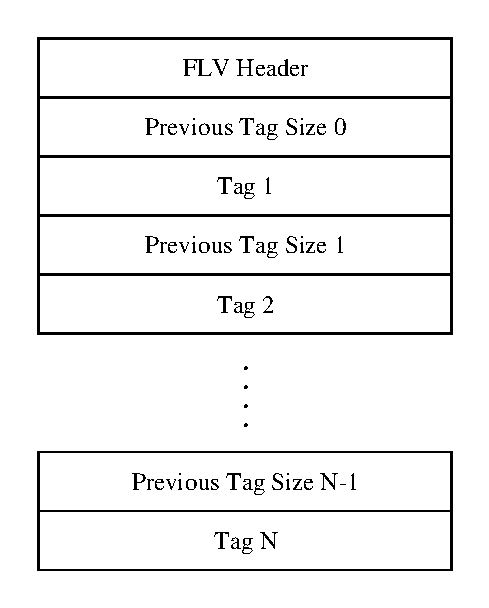
\includegraphics[scale=1]{./Figure/IMG_flv_file.pdf}
    \caption{FLV文件组成结构}
    \label{Fig:flv_file}
\end{figure}

% HTTP-FLV 是基于HTTP进行数据传输的,可以使用HTTP协议的公共端口80,
% 因此可以有效避免出现被防火墙拦截的情况。
% 此外,还可以通过Nginx等软件实现负载均衡,减轻服务端的压力,进行流量的灵活调度。
% 对于需要数据加密的场景,可以通过HTTPS实现。
% 同时它还能很好的支持HTML5,只需要使用 <video> 标签就可以实现在网页中播放HTTP-FLV 视频流。

% 但是由于它的传输特性,浏览器会缓存部分的流媒体资源在本地客户端,在保密性方面存在问题。

%HTTP-FLV 依靠 MIME 的特性,根据协议中的 Content-Type 来选择
%相应的程序去处理相应的内容,使得流媒体可以通过 HTTP 传输。相较于 RTMP 
%协议,HTTP-FLV 能够好的穿透防火墙,它是基于 HTTP/80 传输,有效避免被
%防火墙拦截。除此之外,它可以通过 HTTP 302 跳转灵活调度/负载均衡,支持使
%用 HTTPS 加密传输,也能够兼容支持 Android,iOS 的移动端。

% 说了这么多优点,也来顺便说下 HTTP-FLV 的缺点,由于它的传输特性,。
% 会让流媒体资源缓存在本地客户端,在保密性方面不够好。因为网络流量较
% 大,它也不适合做拉流协议。

\subsection{基于HLS的流媒体传输技术}
HLS协议是由苹果公司在2009年提出的基于HTTP的流媒体传输协议,主要应用于PC端和苹果终端,
可以提供近似实时的流媒体服务,苹果公司在iPhone3.0中首次尝试了该技术\cite{魏雪飞2020HLS}。

HLS协议的原理是将输入的是流切分成若干个小的文件,然后通过一个索引文件将它们串联起来。
播放器需要播放时,会先请求索引文件,再根据索引文件从文件服务器上获对应的音视频等多媒体文件。
其工作原理如图 \ref{Fig:hls} 所示。

\begin{figure}[ht]
    \centering
    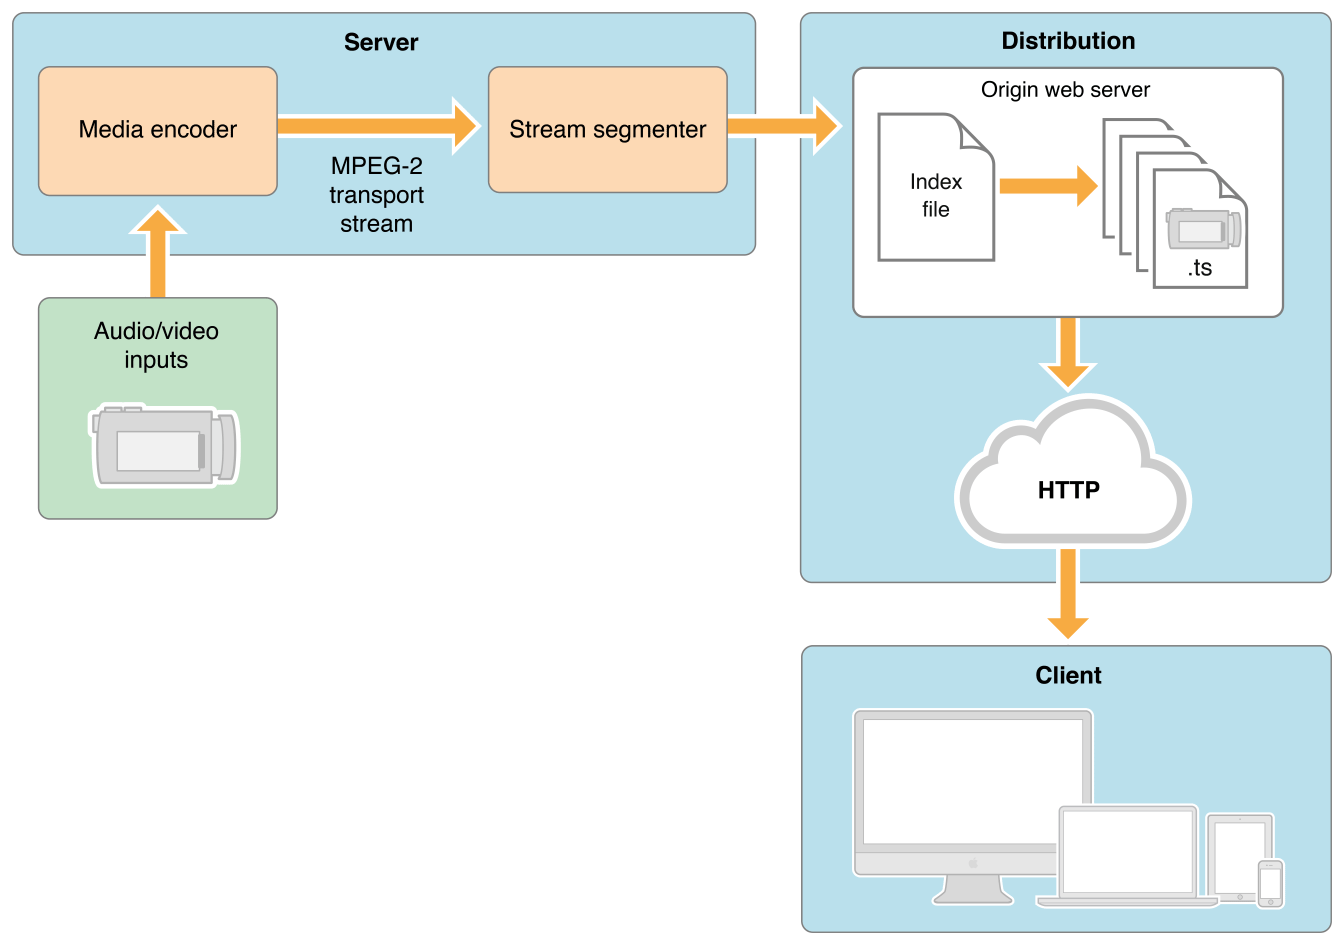
\includegraphics[width=1\linewidth]{./Figure/IMG_hls.png}
    \caption{HLS协议工作原理}
    \label{Fig:hls}
\end{figure}

在图  \ref{Fig:hls} 中,音视频输入设备产生的数据经过 Media encoder 编码后发送到 Stream segmenter 
进行切分操作。
完成切分操作之后,会产生索引文件和对应的多媒体文件,即图中的index file 和 .ts 文件。
之后客户端可以通过HTTP请求的方式获取索引文件和多媒体文件进行播放。

% HLS也是基于HTTP进行数据传输的,所以同样可以避免被防火墙拦截,支持负载均衡。
% 但是由于它需要对输入流进行切分操作,所以会产生较大的延迟,
% 同时也会产生海量的小文件,对存储和缓存由一定的要求。


%上述两个协议都是有Adobe公司推出的,而下面要讲的 HLS (HTTP Live Streaming) 则是苹果公司基于 HTTP 的流媒体传输协议。主要应用于 iOS 设备,包含(iPhone, iPad, iPod touch) 以及 Mac OSX 提供音视频直播服务和录制内容(点播)等服务。

% 相对于常见的流媒体协议,HLS 最大的不同在于它并不是一下请求完整的数据流。它会在服务器端将流媒体数据切割成连续的时长较短的 ts 小文件,并通过 M3U8 索引文件按序访问 ts 文件。客户端只要不停的按序播放从服务器获取到的文件,从而实现播放音视频。

% 相较 RTMP 而言,使用 HLS 在 HTML5 页面上实现播放非常简单:

% 直接:

% preview

% 或者:

% preview

% HLS 的优势:

% Apple 的全系列产品支持:由于 HLS 是苹果提出的,所以在 Apple 的全系列产品包括 iPhone、 iPad、safari 都不需要安装任何插件就可以原生支持播放 HLS, 现在 Android 也加入了对 HLS 的支持。

% 穿透防火墙。基于 HTTP/80 传输,有效避免防火墙拦截

% 性能高。通过 HTTP 传输, 支持网络分发,CDN 支持良好,且自带多码率自适应,Apple 在提出 HLS 时,就已经考虑了码流自适应的问题。

% HLS 的劣势:

% 实时性差,延迟高。HLS 的延迟基本在 10s+ 以上

% 文件碎片。特性的双刃剑,ts 切片较小,会造成海量小文件,对存储和缓存都有一定的挑战


\newpage
\subsection{RTMP、 HTTP-FLV、 HLS简单对比}
表 \ref{Tab:pcompare} 对RTMP、 HTTP-FLV、 HLS这三种协议在底层传输协议、延迟、使用场景等方面进行了对比。

% \begin{table}[ht]
% \centering
% \caption{RTMP、 HTTP-FLV、 HLS对比\cite{RTMP、HTTP-FLV、HLS,你了解常见的三大直播协议吗}}
% \label{Tab:pcompare}
% \begin{tabular}{cccccc}
%     \toprule
%     协议&底层传输协议&视频封装格式&延迟&数据分段&HTML5\\
%     \midrule
%     RTMP&TCP&flv tag&2秒&连续流&不支持\\
%     HTTP-FLV&HTTP&flv&2秒&连续流&支持\\
%     HLS&HTTP&m3u8&10秒以上&切片&支持\\
%     \bottomrule
% \end{tabular}
% \end{table}

\begin{longtable}[ht]{|c|c|c|c|c|c|}
\caption{RTMP、 HTTP-FLV、 HLS对比\cite{RTMP、HTTP-FLV、HLS,你了解常见的三大直播协议吗}}
\label{Tab:pcompare}\\
\hline
协议&底层传输协议&视频封装格式&延迟&数据分段&HTML5\\
\hline
RTMP&TCP&flv tag&2秒&连续流&不支持\\
\hline
HTTP-FLV&HTTP&flv&2秒&连续流&支持\\
\hline
HLS&HTTP&m3u8&10秒以上&切片&支持\\
\hline
\end{longtable}

RTMP 是为流媒体设计的,许多设备使用的推流协议都是 RTMP,应用范围比较广,同时拥有较低的延时。
但是相比于其他两个个协议,它并不HTML5。

HTTP-FLV 基于 HTTP 的长连接特点进行数据的传输,支持HTML5,具有较低的延时。

% 使用类似 RTMP流式的 HTTP 长连接,需由特定流媒体服务器分发的,兼顾两者的优点
% 。以及可以复用现有 HTTP 分发资源的流式协议。它的实时性和 RTMP 相等,与 RTMP 
% 相比又省去了部分协议交互时间,首屏时间更短,可拓展的功能也更多。

HLS是苹果公司提出的直播协议,在苹果的生态系统占据着首要地位,不需要安装任何应用就可以实现播放。
但是与其他两个相比,最致命的缺点就是具有很高的延时。

综上所述,本系统将采用HTTP-FLV协议进行设计和实现。

\section{Spring Boot开发框架}
\subsection{Spring Boot开发框架简介}
Spring Boot框架由Pivotal团队开发,它通过“自动装配”的方式来进行配置,可以省略XML文件的编写,
因此极大程度的简化了基于Spring框架的应用的搭建和开发。
% Spring Boot是由Pivotal团队提供的全新框架,
% 其设计目的是用来简化新Spring应用的初始搭建以及开发过程。
% 该框架使用了特定的方式来进行配置,从而使开发人员不再需要定义样板化的配置。


% Spring Boot不仅继承了Spring框架原有的优秀特性,而且还通过简化配置来进一步简化了Spring应用的整个搭建和开发过程。
在Spring Boot出现之前,使用Spring框架进行应用开发需要编写繁琐的配置文件,然而这些配置文件的内容大多都是类似的。

如图 \ref{Fig:spring} 所示,Spring框架约由20个模块组成,它们被分成
Core Container(核心容器)、
Data Access/Integration(数据访问集成)、
Web(网页)、
AOP(面向切面编程)、
Instrumentation(加载引入)、
Messaging(消息)
和Test(测试)七个大模块。

\begin{figure}[ht]
    \centering
    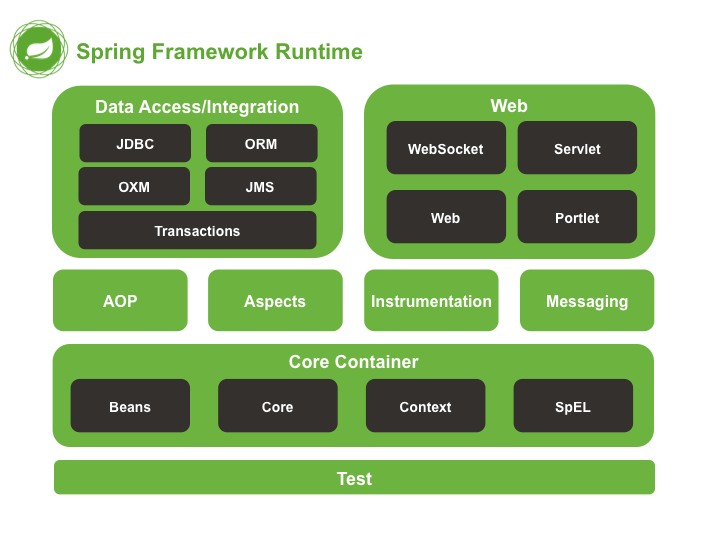
\includegraphics[width=0.8\linewidth]{./Figure/IMG_spring.png}
    \caption{Spring框架模块结构}
    \label{Fig:spring}
\end{figure}

\begin{enumerate}
    \item Core Container 模块是 Spring 框架的基础,提供了控制反转(IoC)和依赖注入(DI)的能力。
    其内部的 BeanFactory 帮助开发者消除了手动创建单例的过程,将单例的创建和组装从业务代码中解耦。
    开发者可以通过ApplicationContext提供的接口访问容器内的创建的对象。
    容器同时还提供了表达式计算、第三方框架集成的能力。
    \item AOP and Instrumentation 模块提供了提供了面向切面编程以及第三方模块集成的能力。
    开发者可以通过面向切面编程可以通过方法拦截器或切点将非业务代码从业务代码中解耦。
    \item Messaging 模块提供了使用消息队列的统一接口。
    \item Data Access/Integration 模块由JDBC、ORM、OXM、JMS和Transaction构成。
    提供了屏蔽数据库供应商的数据库访问接口,并且支持事物。对象映射支持ORM、OXM等映射方式。
    同时还封装了面向消息队列的接口,支持对消息的生产和消费。
    \item Web 模块 提供了面向Web开发的基本功能的集成,例如基于其的Servlet加载、文件上传等功能。
    Web开发能力。可以借助该模块设计并实现一个基于MVC设计模式的Web应用程序。
    \item Test 模块提供了单元测试和集成测试的能力,使得普通的单元测试和集成测试也能使用Spring的容器。
\end{enumerate}

\subsection{控制反转和依赖注入特性简介}
Spring框架具有控制反转(IOC)特性,它通过对象元数据配置文件,借助Java反射机制提供的能力,
将程序生命周期周内的对象的创建和使用统一收口到Spring的容器中,由这个容器进行管理。

控制反转在大多数时候都是通过依赖注入来实现的。当对象A持有了类B的一个实例,就可以说对象A依赖对象B。
依赖注入要求对象与对象之间的依赖仅仅通过构造函数、工厂方法和属性写入方法来定义。

Spring容器就可以将通过这种方式声明的被依赖对象从容器中找到并且通过构造函数、工厂方法和属性写入方法来注入
到需要它的对象内。因为这个被依赖对象的创建过程是由容器完成的并在需要它的时候才进行注入,
而不是被需要它对象的创建的,所以这个过程就体现了控制反转和依赖注入。

在Spring框架的定义中,控制反转又被称为依赖注入。
如图 \ref{Fig:container} 所示,Spring框架会通过对象元数据配置文件和
开发者编写的 POJOs(Plain Old Java Objects)来构造Spring容器,进而启动一个完备的系统。

\begin{figure}[ht]
    \centering   
    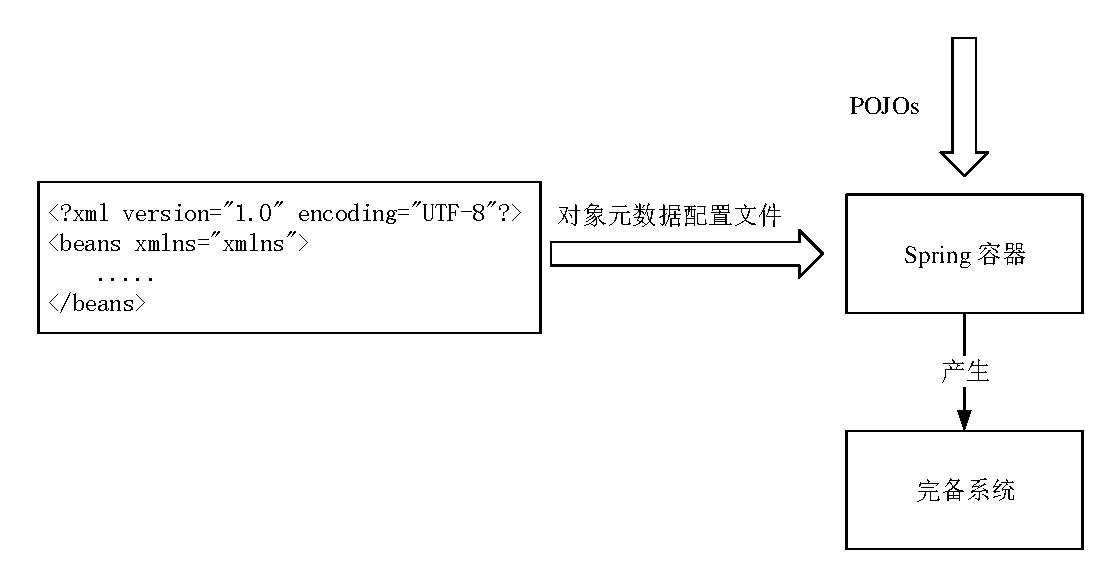
\includegraphics[width=1\linewidth]{./Figure/IMG_container.pdf}
    \caption{IoC和DI工作过程}\label{Fig:container}
\end{figure}

\subsection{面向切面编程简介}
面向切面编程(AOP)可以理解是面向对象编程(OOP)的扩展。
面向切面编程引入,使得面向对象编程具有更高扩展性和更低的耦合性。
面向对象编程中最重要的概念就是对象(Class),而在面向切面编程中,它变成了切面(Aspect)。

在Spring框架中,AOP是最重要的组成部分之一。在AOP中,有一下几个重要的概念:
\begin{enumerate}
    \item 连接点(Join point):程序执行过程中的一个时间点,例如方法执行、异常处理、变量赋值等等。
    在Spring AOP 中,只能是方法执行。
    \item 增强(Advice):在某个特定的连接点上执行的一段额外逻辑。
    可以是在连接点之前、之后或者环绕执行。在多数的AOP框架中,
    是通过拦截器(Interceptor)来实现的,并维护者一个拦截器链。
    \item 切点(Pointcut):是一个谓词表达式,用来计算是否匹配这个连接点。
    对于方法执行的连接点,切点可以是“当参数为某一指定值”。
    \item 切面(Apsect):切面是切点和增强的组合。
\end{enumerate}

在程序执行的过程中,有若干个连接点,每个连接点都可以成为Aspect的目标。

\newpage
AOP的最终目标就是在程序运行的某一个时间点,可以执行一段额外的逻辑。图 \ref{Fig:aop} 
简单描述了AOP的原理和执行过程。
在图 \ref{Fig:aop} 中,切面(Aspect)对应的连接点(Join point)为$Join\ point\ N$,
切点(Pointcut)的谓词表达式为$ pointcut\ ==\ Join\ point\ N$
,而增强(Advice)是在$Code\ N$ 执行之前输出 before,执行之后输出 after。

\begin{figure}[ht]
    \centering   
    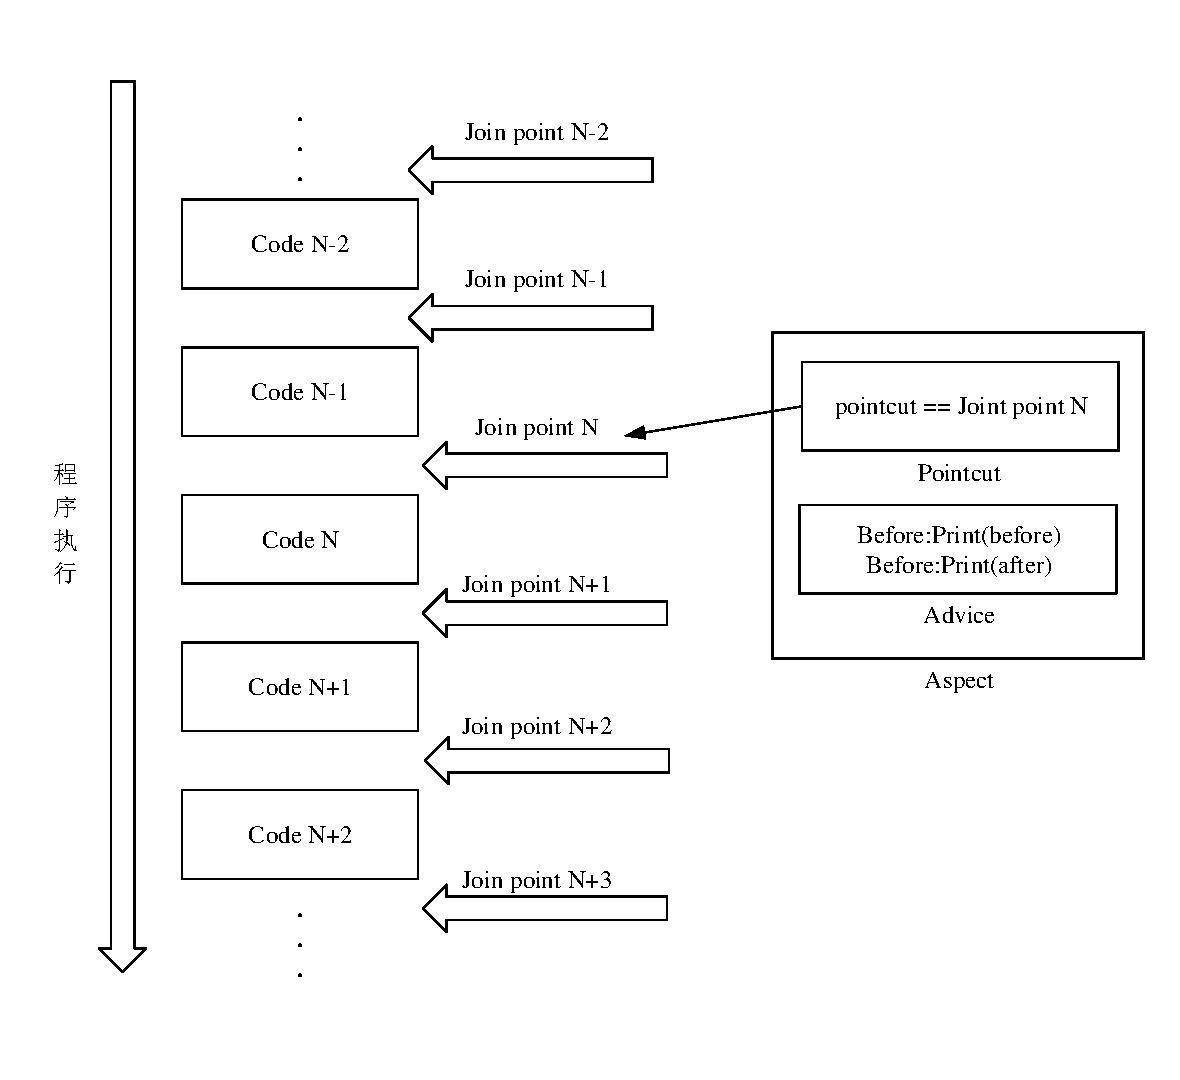
\includegraphics[width=1\linewidth]{./Figure/IMG_aop.pdf}
    \caption{AOP原理示意图}\label{Fig:aop}
\end{figure}

% 的结果就是
% Spring框架具有面向切面编程(AOP)框架,SpringAOP框架基于代理模式,同
% 时运行时可配置;AOP框架主要针对模块之间的交叉关注点进行模块化。

% \section{对象拷贝技术MapStruct}
% TBD
% \section{内存数据库Redis}
% TBD
% \section{RBAC权限系统}
% TBD
\section{本章小结}
本章介绍了系统设计过程中涉及到的关键技术。
首先对流媒体传输技术进行了详细介绍,分析比较了RTMP、HTTP-FLV和HLS三个流媒体传输协议。
紧接着对开发框架Spring Boot的功能和特性进行了介绍。
\chapter{系统需求分析与总体设计}

\section{需求分析}

%本章将详细阐述系统的总体设计。
%对毕业设计题目分析调研过后,可以将设计需求拆分为一下五点。
% 需求分析也称为软件需求分析、系统需求分析或需求分析工程等,
% 是开发人员经过深入细致的调研和分析,准确理解用户和项目的功能、性能、可靠性等具体要求,
% 将用户非形式的需求表述转化为完整的需求定义,从而确定系统必须做什么的过程。\cite{demand_analysis}

本节将从功能性需求和非功能性需求两个角度进行阐述,
前者确定系统需要的功能,后者确定系统的扩展性和兼容性。

\subsection{功能性需求}
本系统的主要目标是设计并实现一个基于Spring Boot的视频实时监控系统,其核心功能是使用户能够
通过登陆访问本系统,并在可见权限范围内进行实时监控视频查看和回放视频查看。在此基础上,
系统引入了一个基于RBAC设计的权限系统,用户可以拥有不同的角色,每个角色可以拥有不同的权限,
这些权限可以包括功能权限、菜单权限等等。

图 \ref{Fig:case} 是系统用户用例图,体现了系统的大致功能。
\begin{figure}[ht]
    \centering   
    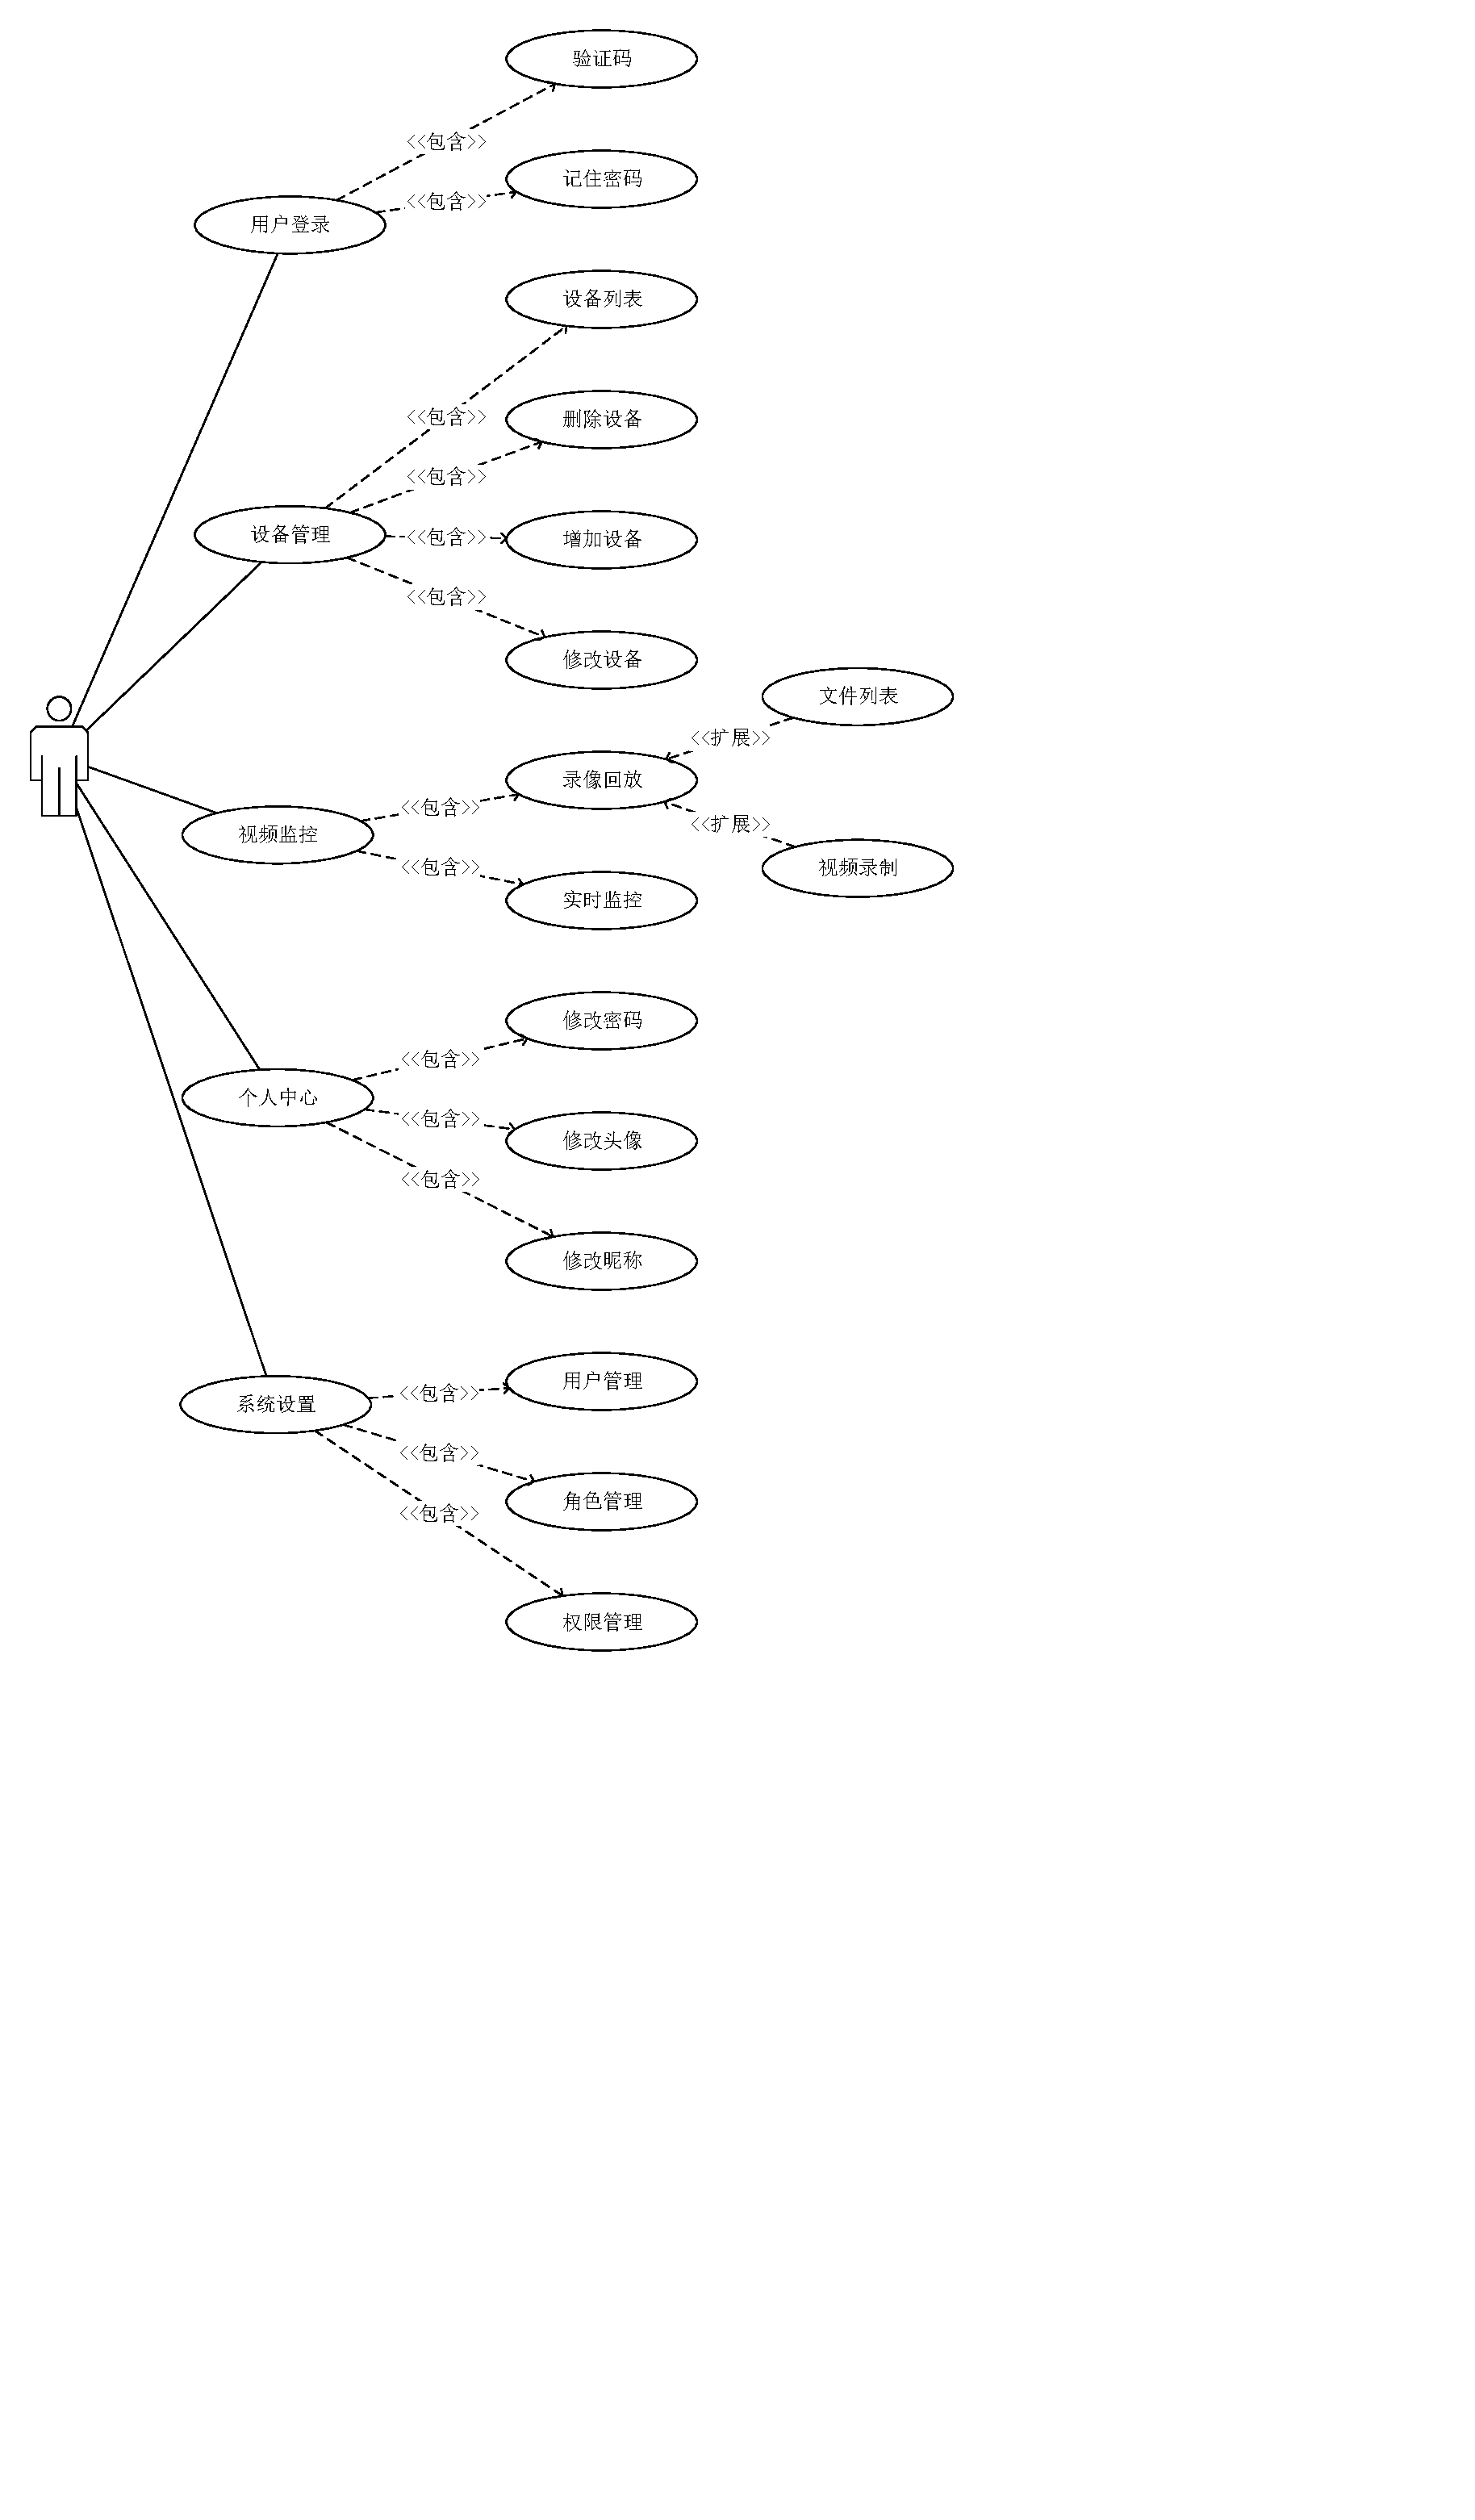
\includegraphics[width=1\linewidth]{./Figure/IMG_case.pdf}
    \caption{系统用户用例图}\label{Fig:case}
\end{figure}

\subsubsection{用户登陆}
在本系统中,用户必须完成登陆才能继续使用,
用户能看到的设备列表信息和视频文件信息都是在当前登陆用户的可见范围内的数据。
在登陆时,用户需要正确输入用户名、密码和图形验证码才能顺利登陆。
如果用户选择了记住密码选项,则下次登陆时就不需要再次输入用户名和密码。

此部分的用例描述如表 \ref{Tab:login} 所示。

\begin{longtable}[ht]{|l|l|}
\caption{用户登录用例描述}
\label{Tab:login}\\
\hline
用例名称&用户登录\\
\hline
用例标识号&Login\\
\hline
参与者&用户\\
\hline
前置条件&无\\
\hline
\multirow{4}*{基本事件流}&1. 用户打开系统登陆页面\\
&2. 用户输入用户名、密码和图形验证码\\
&3. 用户点击登陆按钮\\
&4. 提示登陆成功,跳转到系统主界面\\
\hline
其他事件流&在点击登陆按钮之前,用户名、密码、验证码输入框都不能为空\\
\hline
\multirow{2}*{异常事件流}&1. 提示错误信息\\
&2. 更新验证码\\
\hline
后置条件&系统进入主界面,选择记住密码后用户名和密码保存到本地\\
\hline


% \multicolumn{2}{|c|}{ \multirow{2}*{$S_i$} }& \multicolumn{4}{c|}{事件} &\multirow{2}*{max}\\
% \cline{3-6}
% \multicolumn{2}{|c|}{}&50&100&150&200&\\
% \hline
% \multirow{4}*{策略}&50&0&100&200&300&300\\
% \cline{2-7}
% &100&100&0&100&200&200\\
% \cline{2-7}
% &150&200&100&0&100&200\\
% \cline{2-7}
% &200&300&200&100&0&300\\
% \end{tabular}
\end{longtable}

\newpage
\subsubsection{设备管理}

设备管理部分会展示设备列表,其中包括了当前登陆用户可见的所有设备。
用户可以根据设备名称和设备类型进行搜索筛选,支持分页查询。
用户可以进行设备的增加、修改和删除操作。被删除的设备不会从列表中消失,仅仅只是更改“删除状态”。

此部分的用例描述如表 \ref{Tab:device} 所示。

\begin{longtable}[ht]{|l|l|}
    \caption{设备管理用例描述}
    \label{Tab:device}\\
\hline
用例名称&设备管理\\
\hline
用例标识号&Device\\
\hline
参与者&用户\\
% \hline
% 简要说明&用例变好\\
\hline
前置条件&用户已经登陆,拥有相关菜单权限和数据权限\\
\hline
\multirow{4}*{基本事件流}&1. 用户进入设备列表页面,可以翻页查看、条件搜索。\\
&2. 用户更改设备删除状态,对设备进行删除和恢复\\
&3. 用户点击添加按钮,填写设备相关信息后提交完成添加\\
&4. 用户点击修改按钮,弹出对话框,更改信息后提交完成修改\\
\hline
其他事件流&在添加设备、修改设备时,用户填写的数据必须符合要求\\
\hline
\multirow{2}*{异常事件流}&1. 提示信息填错错误\\
&2. 用户重新填写后再次提交\\
\hline
后置条件&无\\
\hline
\end{longtable}

\newpage
\subsubsection{视频监控}
视频监控包含录像回放和实时监控。
用户可以在录像回放下查看所有未被删除和被删除的设备的历史监控视频文件,可以在线播放和下载。
实时监控可以查看未被删除的设备的实时监控视频。

此部分的用例描述如表 \ref{Tab:video} 所示。

\begin{longtable}[ht]{|l|l|}
    \caption{视频监控用例描述}
    \label{Tab:video}\\
\hline
用例名称&视频监控\\
\hline
用例标识号&Video\\
\hline
参与者&用户\\
% \hline
% 简要说明&用例变好\\
\hline
前置条件&用户已经登陆,拥有相关菜单权限和数据权限\\
\hline
\multirow{5}*{基本事件流}&1. 用户选择录像回放功能,展示文件列表,支持搜索和分页查询\\
&2. 在文件列表中可以选择任意文件进行在线播放和下载\\
&3. 用户选择实时监控功能,展示设备列表\\
&4. 在设备列表中可以选择未被删除的设备进行实时监控视频的查看\\
&5. 后台持续进行设备的视频录制\\
\hline
其他事件流&无\\
\hline
异常事件流&无\\
\hline
后置条件&无\\
\hline
\end{longtable}

\newpage
\subsubsection{个人中心}
个人中心只要包括用户信息的展示和修改。只有用户的头像、密码和昵称支持修改。

此部分的用例描述如表 \ref{Tab:info} 所示。

\begin{longtable}[ht]{|l|l|}
    \caption{个人中心用例描述}
    \label{Tab:info}\\
\hline
用例名称&个人中心\\
\hline
用例标识号&Info\\
\hline
参与者&用户\\
% \hline
% 简要说明&用例变好\\
\hline
前置条件&用户已经登陆,拥有个人中心的菜单权限和数据权限\\
\hline
\multirow{3}*{基本事件流}&1. 用户选择图片进行上传,更改头像\\
&2. 用户修改用户昵称和密码\\
&3. 点击提交按钮完成修改\\
\hline
其他事件流&用户头像、昵称和密码的修改需要符合规范\\
\hline
\multirow{2}*{异常事件流}&1. 提交无效的数据,提示相关错误信息\\
&2. 用户修正后重新提交\\
\hline
后置条件&无\\
\hline
\end{longtable}

\newpage
\subsubsection{系统设置}
系统设置主要是对权限相关的部分进行操作。具有这部分权限的用户可以对系统用户进行增删改查,
增加系统角色系统权限,对用户和角色、角色和权限进行关联。

此部分的用例描述如表 \ref{Tab:system} 所示。

\begin{longtable}[ht]{|l|l|}
    \caption{系统设置用例描述}
    \label{Tab:system}\\
\hline
用例名称&系统设置\\
\hline
用例标识号&Syetem\\
\hline
参与者&用户\\
% \hline
% 简要说明&用例变好\\
\hline
前置条件&用户已经登陆,拥有系统设置的菜单权限和数据权限\\
\hline
\multirow{6}*{基本事件流}&1. 用户打开系统设置界面\\
&2. 在用户列表可以对用户进行增删改查\\
&3. 在角色列表可以进行角色的增删改查\\
&4. 在权限列表可以进行权限的增删改查\\
&5. 在角色列表选择角色之后,可以关联权限到该角色上\\
&6. 在用户列表选择用户之后,可以关联角色到该用户上\\
\hline
其他事件流&在进行关联、修改数据等操作时,需要符合数据规范\\
\hline
\multirow{2}*{异常事件流}&1. 提交数据不符合规范,提示错误信息\\
&2. 用户修正信息后重新提交\\
\hline
后置条件&无\\
\hline
\end{longtable}

\newpage
\subsection{非功能性需求}
\subsubsection{兼容性}
系统基于设备的 HTTP-FLV直播流进行实时监控查看和历史视频查看,
屏蔽了不同厂商设备底层的差异,只要设备能提供HTTP-FLV地址,就可以在本系统中添加使用。

\subsubsection{数据完整性}
在进行监控视频录制时,会冗余部分视频数据,这样在某一段时间的视频文件丢失时,
可以在这段时间之前和之后的视频文件中找到。

\section{系统数据库设计}
本系统借助MySQL数据库进行数据的存储和管理。
MySQL是关系型数据库,需要先通过E-R图来展示系统之间各个实体的属性和它们之间的联系。
然后再借助 E-R图,完成数据表的设计。
系统的实体关系图如图 \ref{Fig:erd} 所示,因为篇幅限制,只展示了实体的部分核心属性。

\begin{figure}[ht]
    \centering
    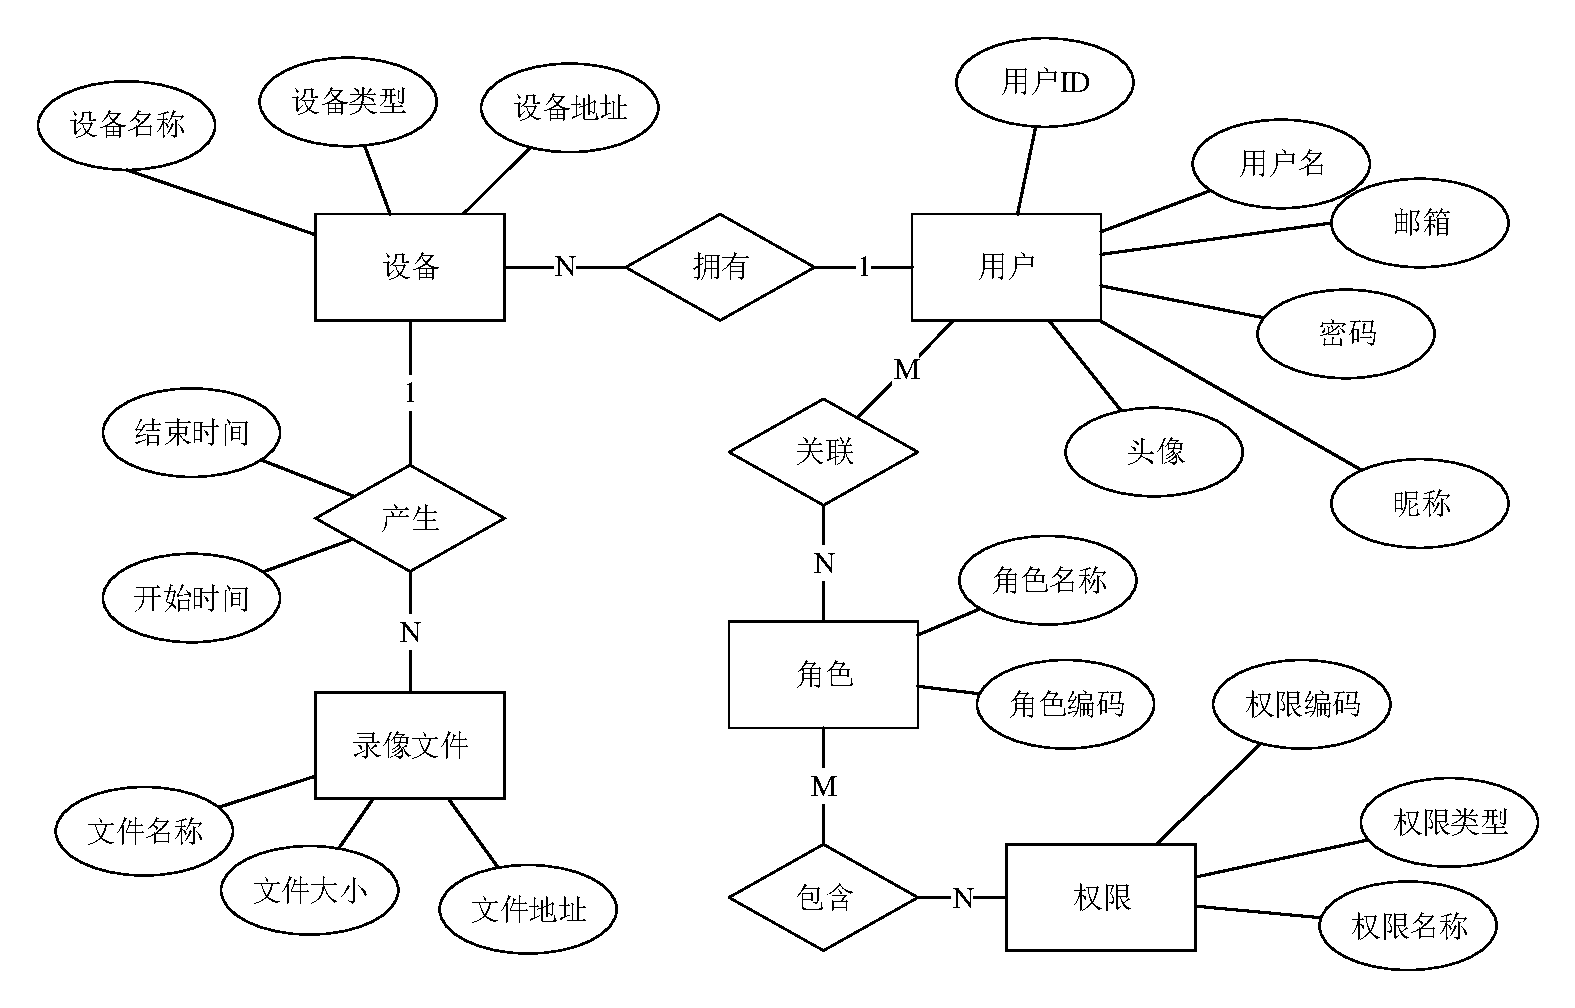
\includegraphics[width=0.8\linewidth]{./Figure/IMG_er.pdf}
    \caption{实体关系图}\label{Fig:erd}
\end{figure}

% 一个完整的系统必然设计到用户,因此就需要用户实体。
% 由于是视频监控系统,那么有监控摄像头设备,因此需要设备实体。
% 此外还需要对监控摄像头产生的录像文件进行保存并支持检索,所以需要视频文件实体。

% 综上所示,本视频实时监控系统包括三个实体:用户、设备和视频文件。
% 本

% 通过实体关系图,可以推导出数据库表结构和表关系,同样如下图所示。

% 根据 图 \ref{Fig:erd} ,可以推导出数据库中数据表的结构,下面列出了数据库中部分关键的数据表。

% \begin{figure}[ht]
%     \centering
%     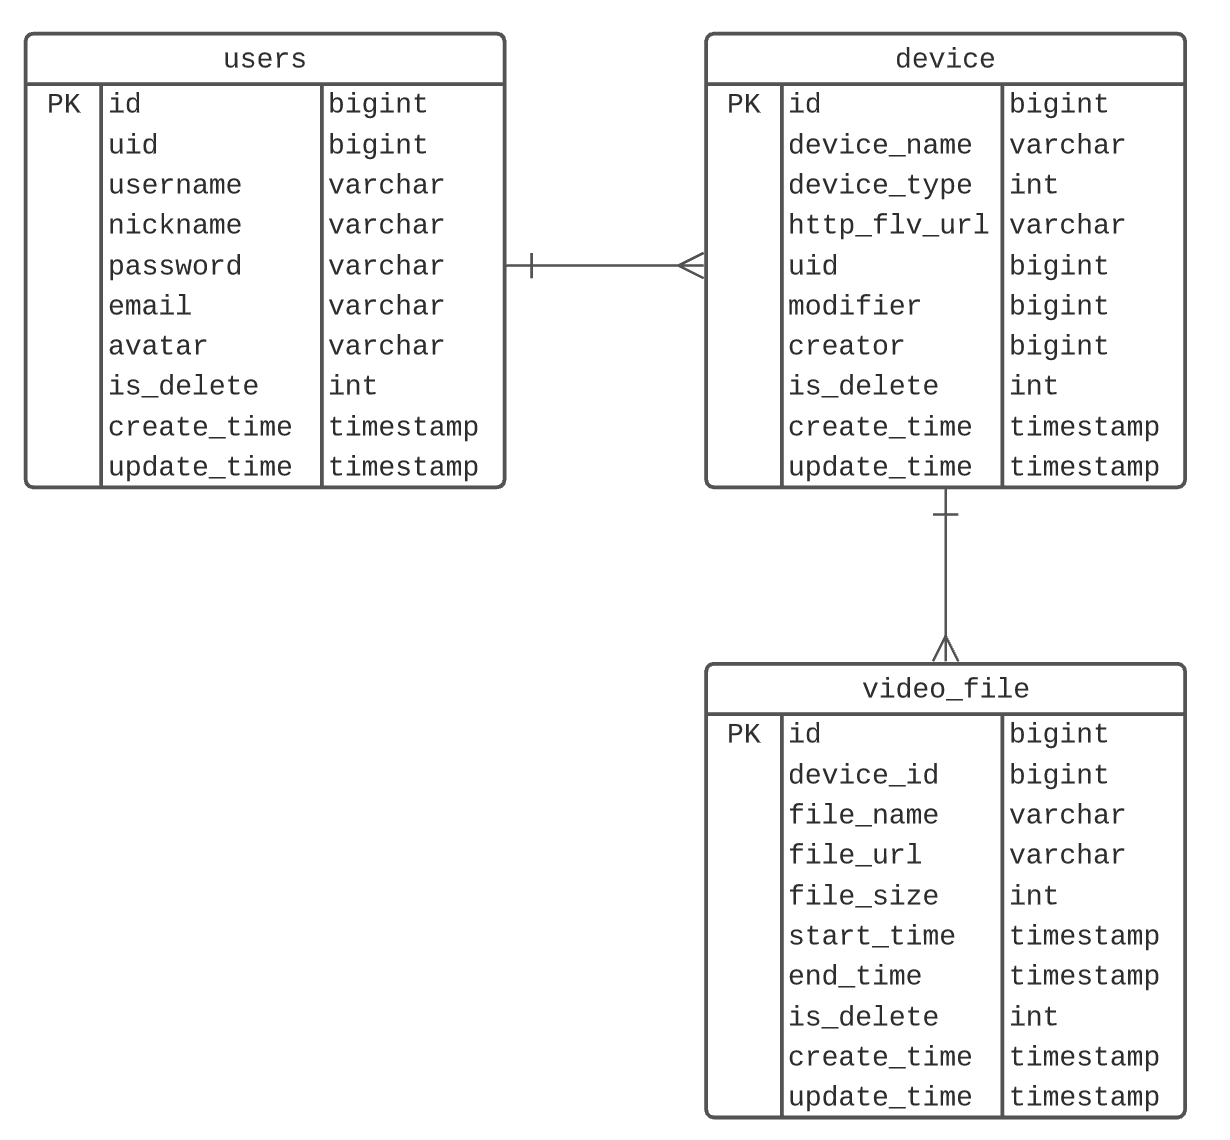
\includegraphics[scale=.6]{./Figure/IMG_db.png}
%     \caption{数据库表结构和表关系}\label{Fig:db}
% \end{figure}

% \section{交互接口设计}

\section{系统架构设计}
本系统架构设计分为五个模块,如表 \ref{Tab:module} 和图 \ref{Fig:struct} 所示。
本节将对每个模块的功能做详细介绍。

\begin{longtable}[c]{|C{5cm}|C{7cm}|}
    \caption{系统模块表}\label{Tab:module}\\
    \hline
    模块名称 & 模块功能\\
    \hline
    公共模块&提供公共工具的能力\\ %
    \hline
    数据存储模块&提供持久组件的读写的能力\\ %
    \hline
    业务逻辑模块&系统的主要业务逻辑\\ % 
    \hline
    视频文件存取模块&离线视频文件的存取\\ % 
    \hline
    前端接口交互模块&为前端提供接口交互\\ %
    \hline
\end{longtable}

\begin{figure}[ht]
    \centering
    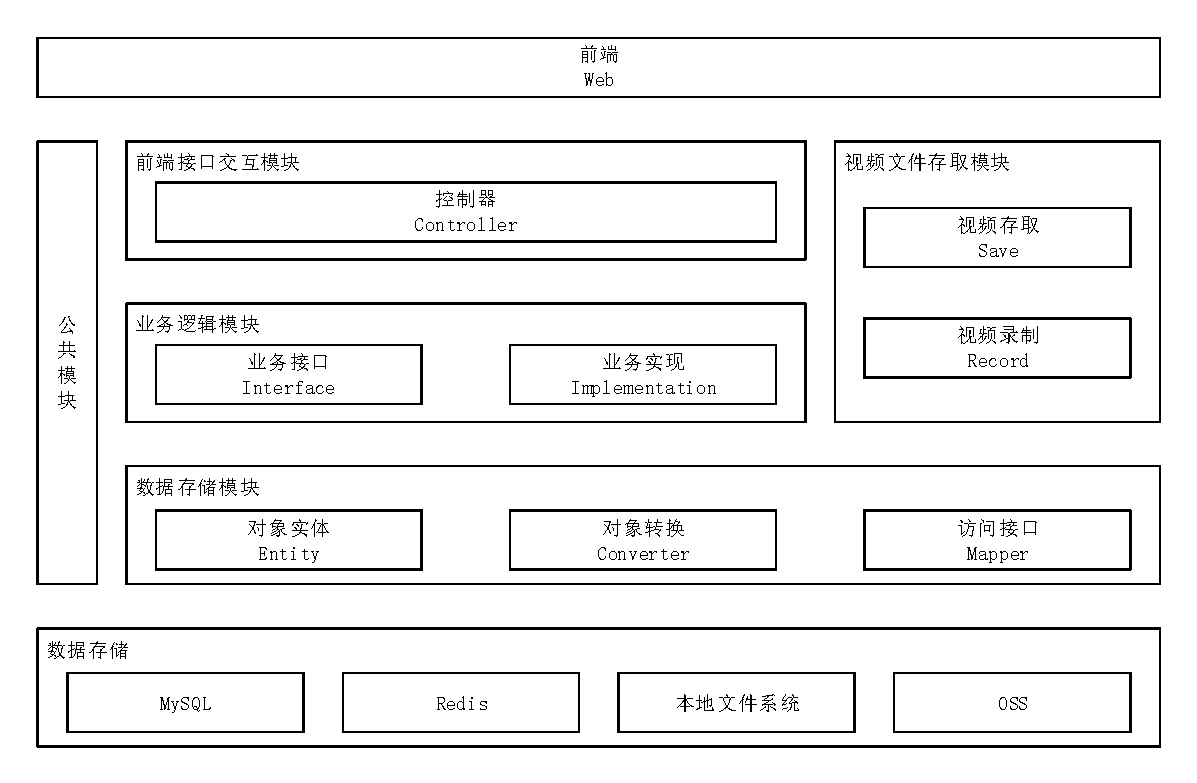
\includegraphics[scale=.7]{./Figure/IMG_struct.pdf}
    \caption{软件总体框架图}\label{Fig:struct}
\end{figure}

\subsection{公共模块}
公共模块(monitoring-system-common)提供公共工具的能力。
模块内主要包括开发过程中需要用到的注解(annotation)、常量(constant)、枚举(enumerate)、
异常(exception)以及公共的工具封装(utility)。

公共模块中封装的工具包括时间转换工具类、HTTP请求工具类、Spring工具类以及登陆验证码工具类。

时间转换工具类提供将java.util.Date对象转为具有一定格式的字符串(例如“yyyy-MM-dd HH:mm:ss”),
同时也提供逆向转换的能力,即将字符串格式的时间转化为java.util.Date对象。
% 为什么需要

HTTP请求工具类封装了HTTP请求中相关的GET、POST两种请求方法,借助第三方依赖OkHttp二次开发实现。
支持带参数的GET请求、带请求体参数的POST请求。

Spring工具类提供了对Spring上下文的ApplicationContext的静态访问,
可以在全局状态下任何一个地方访问上下文,即可以访问容器内管理的对象和使用Spring提供的观察者模式。

登陆验证码工具类主要提供在登录时生产验证码图片,如图 \ref{Fig:code} 所示。

\begin{figure}[ht]
    \centering
    
\includegraphics[width=0.5\linewidth]{./Figure/IMG_code.png}
    \caption{登陆验证码}\label{Fig:code}
\end{figure}

\subsection{数据存储模块}
数据存储模块(monitoring-system-repo)提供持久组件的读写的能力。持久组件就是提供数据存储的服务,
在本系统的设计中,持久组件包括MySQL数据库、Reids内存数据库、本地文件系统。

系统设计使用 Mybatis 框架对数据库进行访问,因此该模块中的大部分代码有时有 Mybatis-Generator
自动生成,包括实体对象类、Mapper接口和Mapper配置文件。除此之外,该模块还包括了各种实体的封装类,
比如前端参数封装类(用于封装前端传递给后端的参数)、HTTP响应类(封装后端接口返回对象)
以及各个模块使用的实体类(VO、BO)。

该模块还负责对象之间的转换,即将VO转换成BO或者将BO转换成BO等。该功能是通过对象拷贝技术MapStruct生成的对象转换代码实现的。

\subsection{业务逻辑模块}
业务逻辑模块(monitoring-system-service)提供业务逻辑处理的功能。
该模块是本系统最核心的一个模块,主要负责业务模块的逻辑应用设计,支持登陆鉴权、设备信息的增删改查、个人信息修改等。

业务逻辑模块的主要设计思路是面向接口编程。
接口主要用于描述类具有什么功能,而并不给出每个功能的具体实现。
一个类可以实现一个或多个接口,并在需要接口的地方,随时使用实现了相应接口的对象。

首先设计接口,再设计其对应的实现的类,接着利用Spring的依赖注入特性,
就可以在上层模块声明接口类型的变量,而无需关心其具体实现。
换句话说,业务逻辑模块的变动不会对上层模块的调用产生任何影响。

这就是软件六大设计原则之一的依赖倒置原则,即面向接口编程。
上层模块不应该依赖底层模块,它们都应该依赖于抽象。
抽象不应该依赖于细节,细节应该依赖于抽象。
上层模块不应依赖底层模块,即上层的业务模块不应该依赖底层的实现模块。
如:人出行使用交通工具,只需要知道是交通工具就可以,不用知道是哪种具体的交通工具。
抽象不应该依赖于细节,细节应该依赖于抽象。
在具体的Java编程中,抽象指代接口、抽象函数,统称为接口,而细节指代接口的具体实现。

\subsection{视频文件存取模块}
视频文件存取模块(monitoring-system-media)提供实时监控视频录制和离线查看检索功能。
该模块提供了两个HTTP的接口,分别是监控回放文件的列表查询接口和监控回放文件下载接口。
对于已经在本系统中绑定的监控摄像头设备,每隔一分钟视频文件存取模块会执行定时任务,
对该设备进行录制,并且录制的时长为80秒,目的是做到前后视频文件能有重合部分,防止视频数据丢失。

对于视频文件的存放,可以在本地文件系统和云存储之间无缝切换。
云存储采用阿里云的OSS对象存储服务或本地搭建的Hadoop分布式存储系统。
对于视频文件的读取,该模块提供了一个GET 方法的HTTP接口,入参为视频文件的名称,返回值为该文件内容。
同时还提供搜索功能,支持按照监控视频的开始时间和结束时间进行范围查找。


\subsection{前端接口交互模块}
前端接口交互模块(monitoring-system-web)提供与前端交互的能力。
该模块负责接受前端的请求,然后调用下层模块(如视频文件存取模块)提供的接口方法,实现业务逻辑,
然后将下层模块的返回值进行一定程度的封装后返回给前端进行展示。


% \subsection{软件总体框架}



% \section{权限系统设计}
% TBD

\section{本章小结}
本章从功能性需求和非功能性需求两方面对系统进行了需求分析,然后介绍了系统的数据库设计和系统架构设计。

\chapter{系统实现和系统测试}
本章将将介绍系统实现和系统测试两大部分。
% \section{开发环境搭建}
% \subsection{前端开发环境搭建}
前端使用 Vue.js 框架进行开发,通过 yarn 和 npm 进行项目依赖管理。开发IDE使用 Visual Code。 
% \subsection{后端开发环境搭建}
后端使用 Spring Boot 框架进行开发,通过 Maven 进行项目依赖管理。开发IDE使用 IDEA。 

\section{前端界面实现}
本系统采用前后端分离的开发模式,因此前端页面与后端服务是完全独立的。
本节将介绍前端界面的实现,主要采用 Element-UI开源组件开发。

\subsection{登陆界面}

登陆界面如图 \ref{Fig:login} 所示,分为三个主要部分:信息输入、图形验证码和按钮。

\begin{figure}[ht]
    \centering
    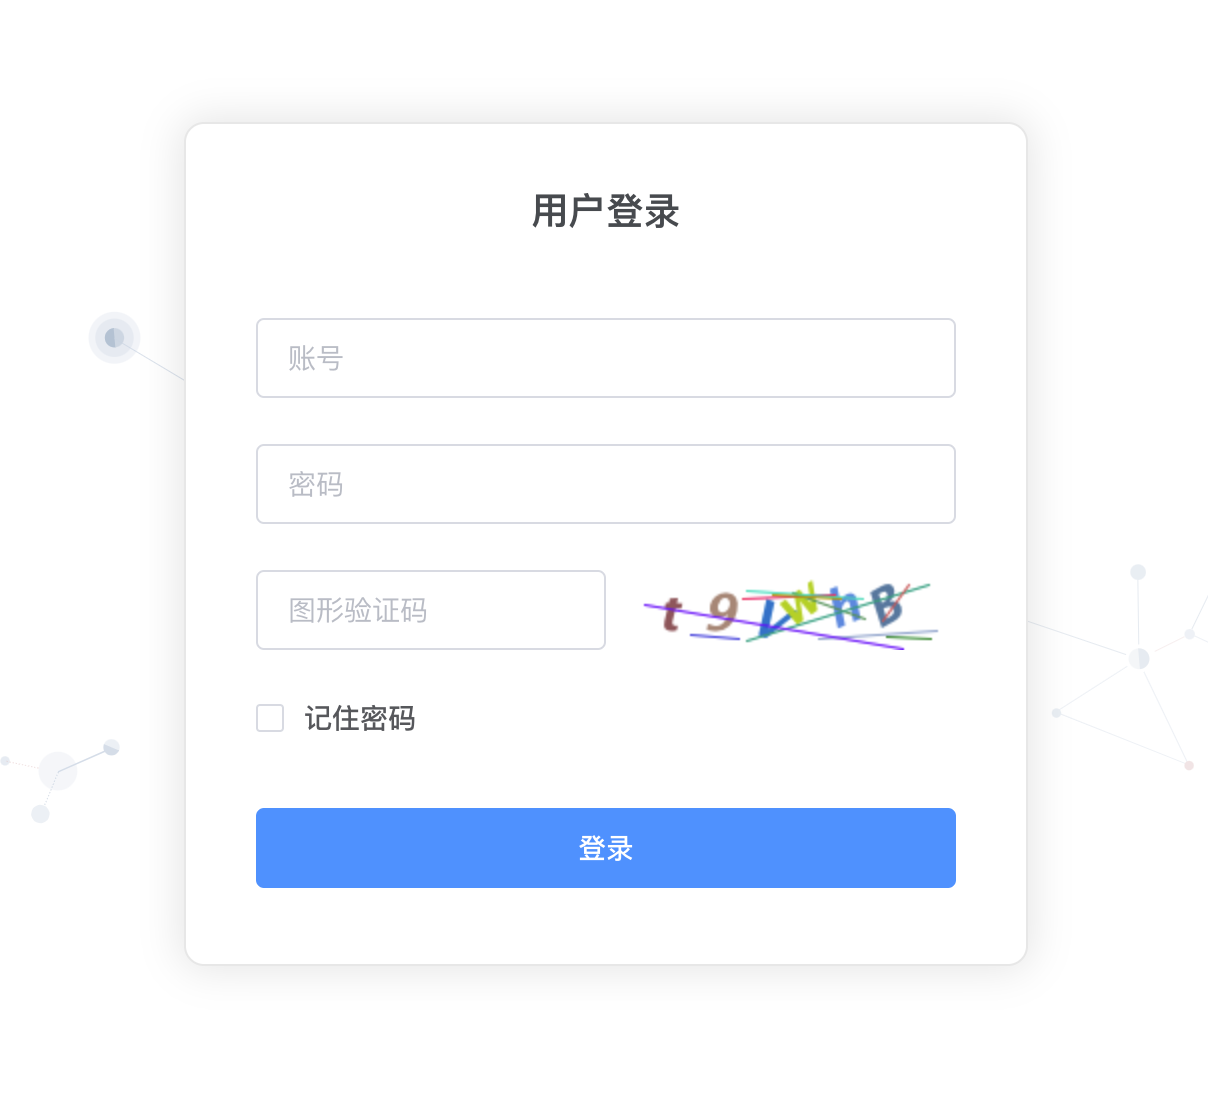
\includegraphics[width=0.8\linewidth]{./Figure/IMG_login.png}
    \caption{登陆页面}\label{Fig:login}
\end{figure}

信息输入部分有三个输入框,分别是用户名输入框、密码输入框、图形验证码输入框和“记住密码”选择框。
图形验证码部分用于展示图形验证码。
登陆按钮用于向服务器提交用户名、密码和图形验证码。
登陆成功之后会跳转到基础管理的设备管理菜单。

\subsection{实时监控播放}
实时监控的播放和监控回放的播放都是通过 Bilibili的开源组件 flv.js 实现的。

数据库中记录这每一台设备的 HTTP-FLV 视频流地址,前端在获取到这个地址后,通过 flv.js 组件
可以在HTML页面中实时播放这个链接,如图 \ref{Fig:record_eg} 所示。

\begin{figure}[ht]
    \centering
    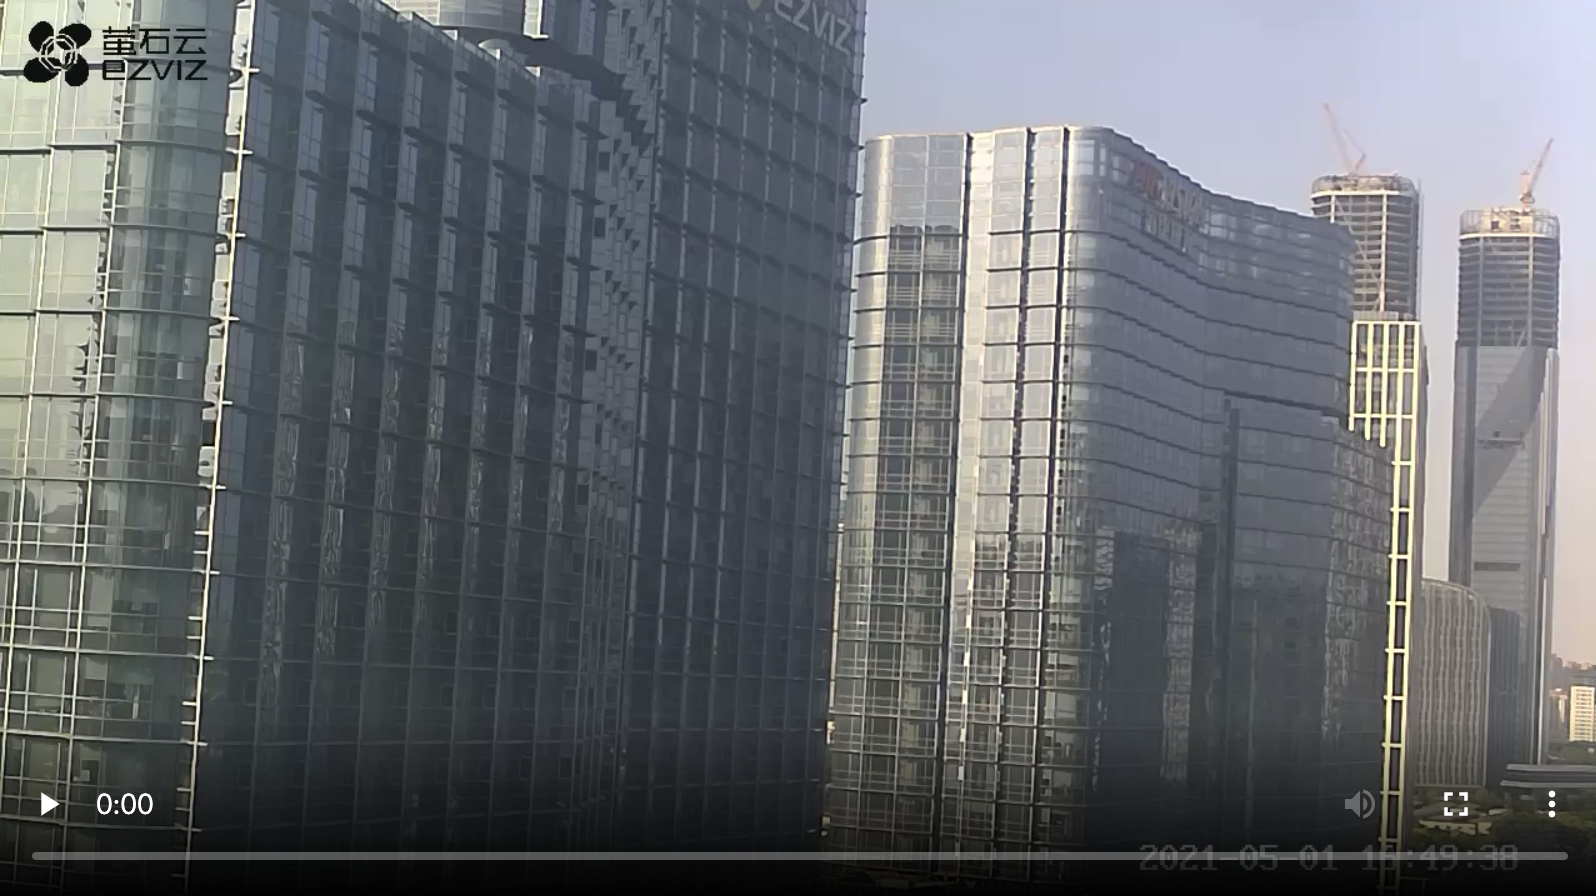
\includegraphics[width=1\linewidth]{./Figure/IMG_record_eg.png}
    \caption{实时监控播放示例}\label{Fig:record_eg}
\end{figure}

\subsection{监控回放播放}
系统会对实时的监控视频进行录制,为了保证数据的完整性,录制视频的有效时长为1分钟,多余的部分为冗余数据。
可以在回放文件的列表中对视频进行在线的播放或者下载到本地,如图 \ref{Fig:file_list} 所示。

\begin{figure}[ht]
    \centering
    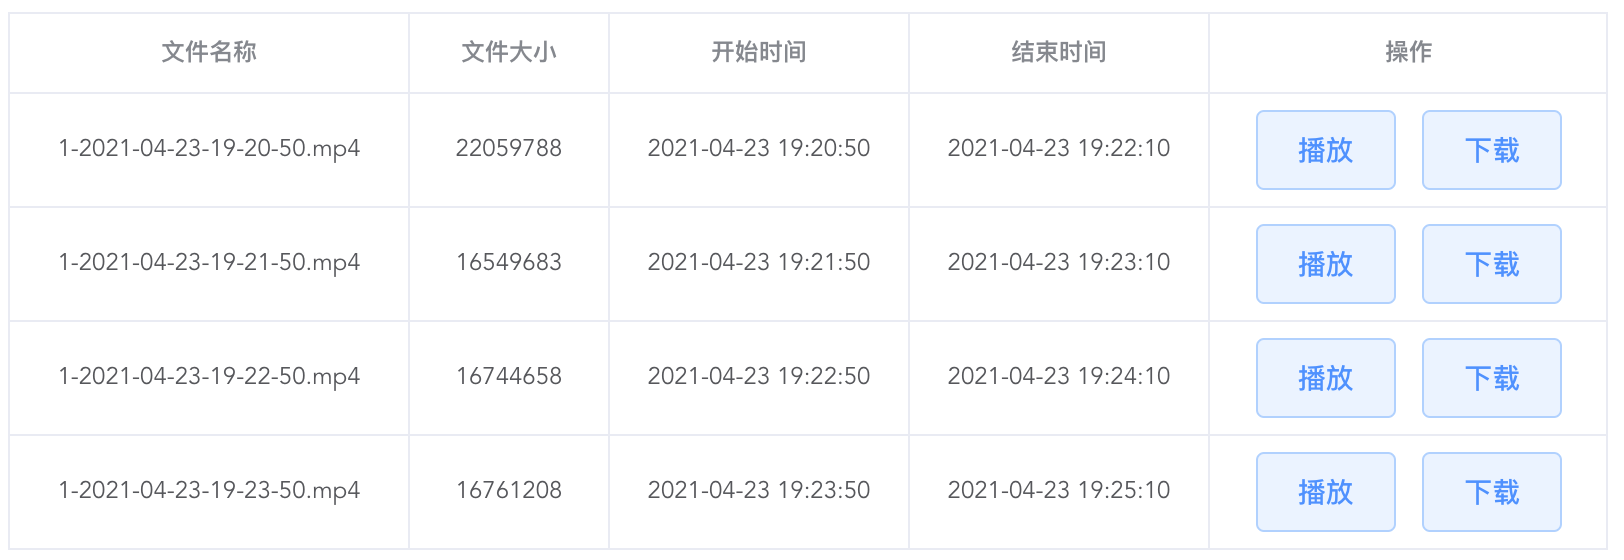
\includegraphics[width=1\linewidth]{./Figure/IMG_file_list.png}
    \caption{监控回放播放示例}\label{Fig:file_list}
\end{figure}

\newpage
\subsection{页面布局}
页面布局分为三个部分:顶部导航栏、左侧菜单栏和主窗口,如图 \ref{Fig:layout} 所示。

\begin{figure}[ht]
    \centering
    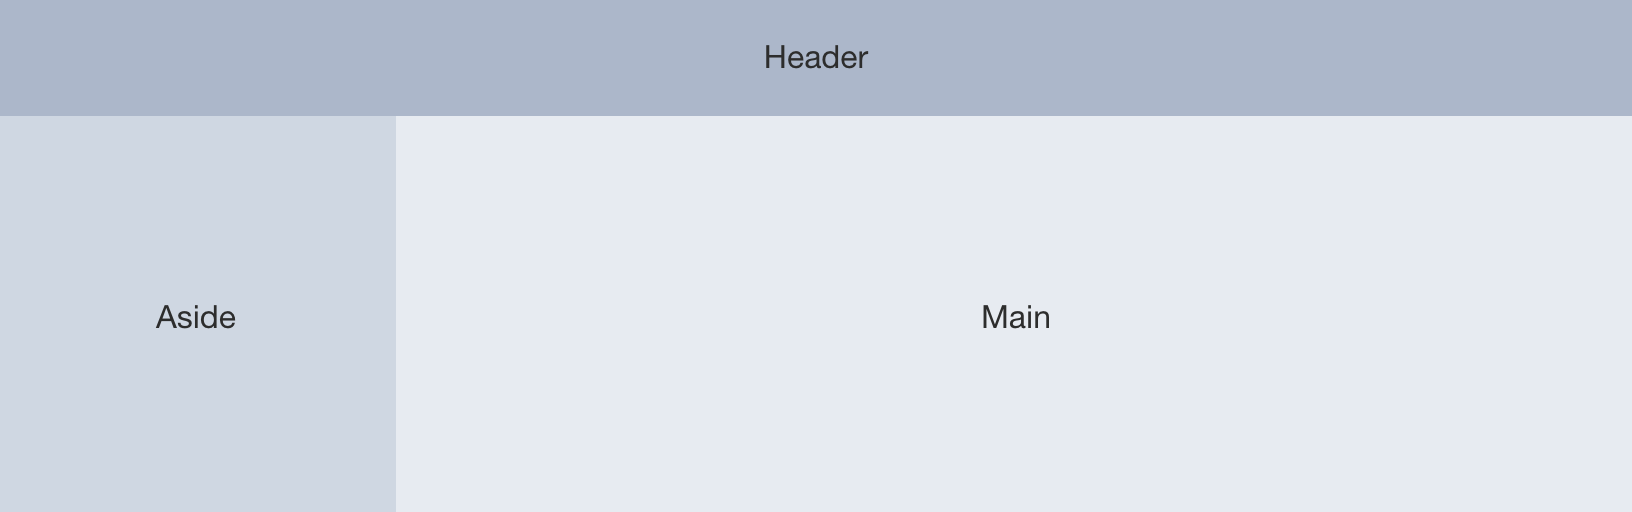
\includegraphics[width=1\linewidth]{./Figure/IMG_layout.png}
    \caption{页面布局}\label{Fig:layout}
\end{figure}

\subsubsection{顶部导航栏}
顶部导航栏使用 Element-UI 中的NavMenu 导航菜单组件开发,
用于展示用户名和头像,可以通过点击用户名或者头像打开下拉菜单,如图 \ref{Fig:top} 所示。

\begin{figure}[ht]
    \centering
    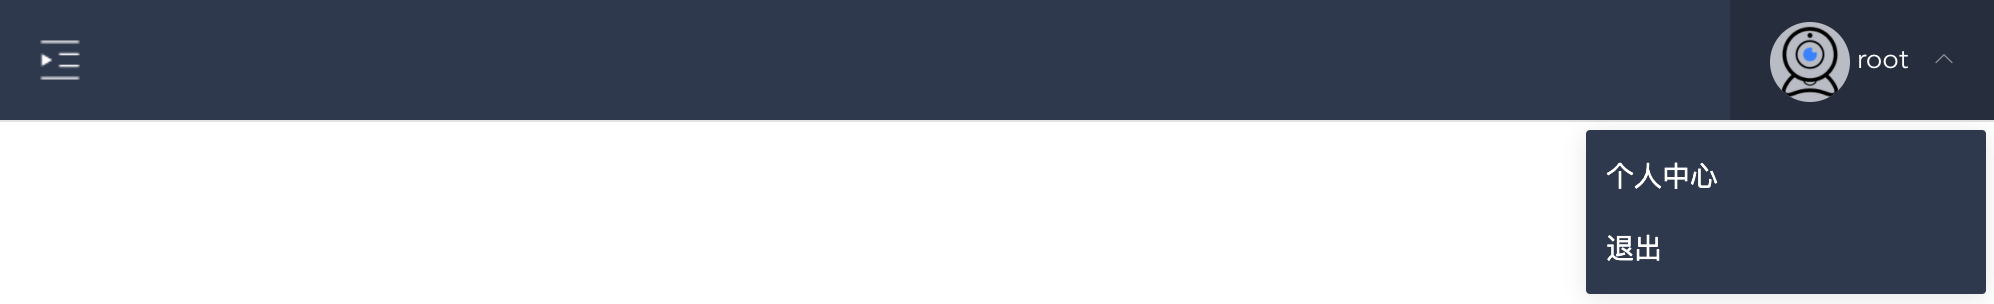
\includegraphics[width=1\linewidth]{./Figure/IMG_top.png}
    \caption{顶部导航栏}\label{Fig:top}
\end{figure}

用户单击个人中心可以跳转到个人中心页面;
用户单击退出会弹出二次确认对话框,选择是后会退出登陆并跳转到登陆页面。

\subsubsection{左侧菜单栏}
系统的总菜单布局在页面的左侧,分为三个一级菜单,每个一级菜单下又有二级菜单,
如图 \ref{Fig:left_menu} 所示。

\begin{figure}[ht]
    \centering
    \subcaptionbox{基础管理菜单}
    {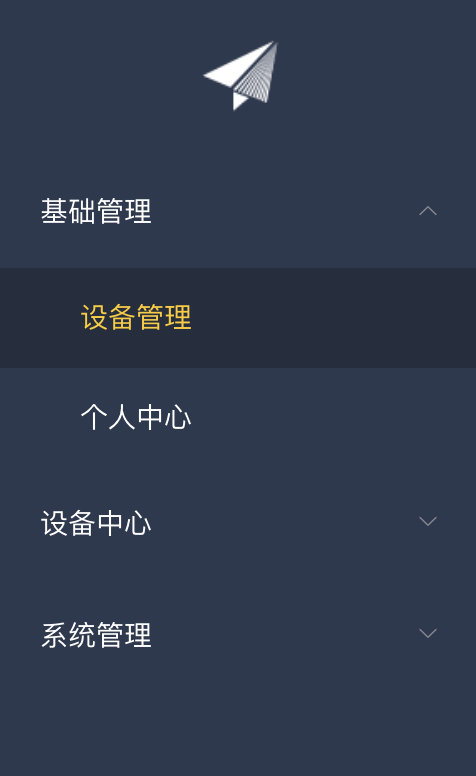
\includegraphics[width=.3\linewidth]{./Figure/IMG_left_menu_1.png}}
    \subcaptionbox{设备中心菜单}
    {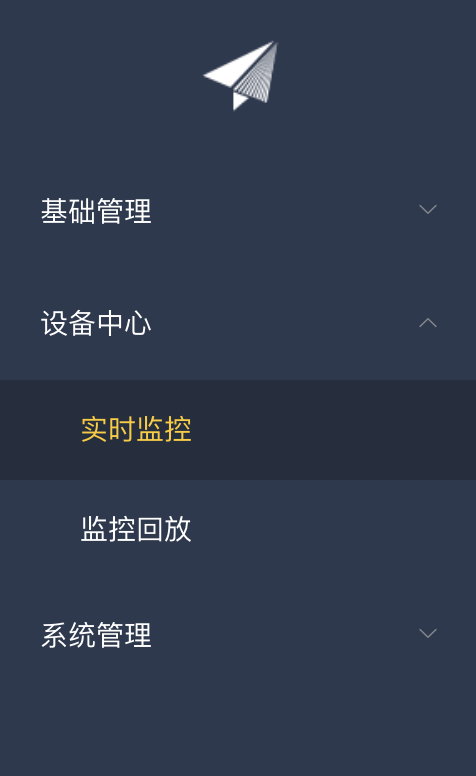
\includegraphics[width=.3\linewidth]{./Figure/IMG_left_menu_2.png}}
    \subcaptionbox{系统管理菜单}
    {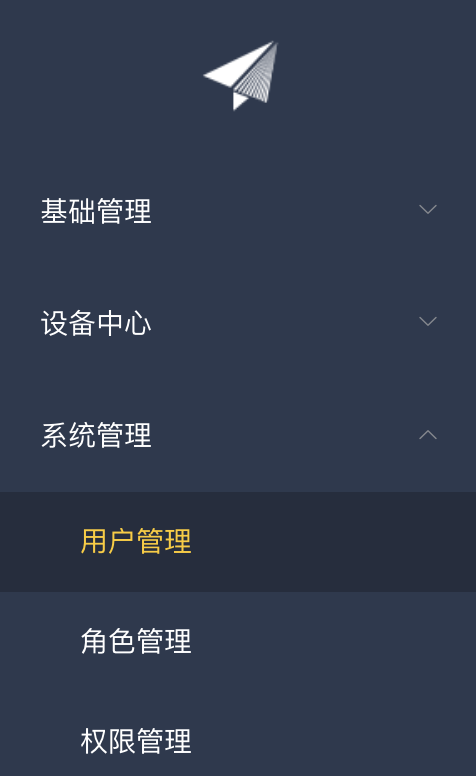
\includegraphics[width=.3\linewidth]{./Figure/IMG_left_menu_3.png}}
    \caption{左侧菜单}\label{Fig:left_menu}
\end{figure}

基础管理菜单下有设备管理菜单和个人中心菜单。
设备中心菜单下有实时监控菜单和监控回放菜单。
系统管理菜单下有用户管理菜单、角色管理菜单和权限管理菜单。

左侧菜单会因为每个用户拥有不同的菜单权限而有不同的展示。
单击对应的菜单可以跳转到对应的页面。

\subsubsection{主窗口}
主窗口会根据不同的二级菜单而展示不同的内容,主要用于承载信息、完成操作。

\newpage
\subsection{二级菜单页面}
各个二级菜单的页面结构大致相同,如图\ref{Fig:main} 所示,主要分为四部分:导航、搜索、列表、分页。

\begin{figure}[ht]
    \centering
    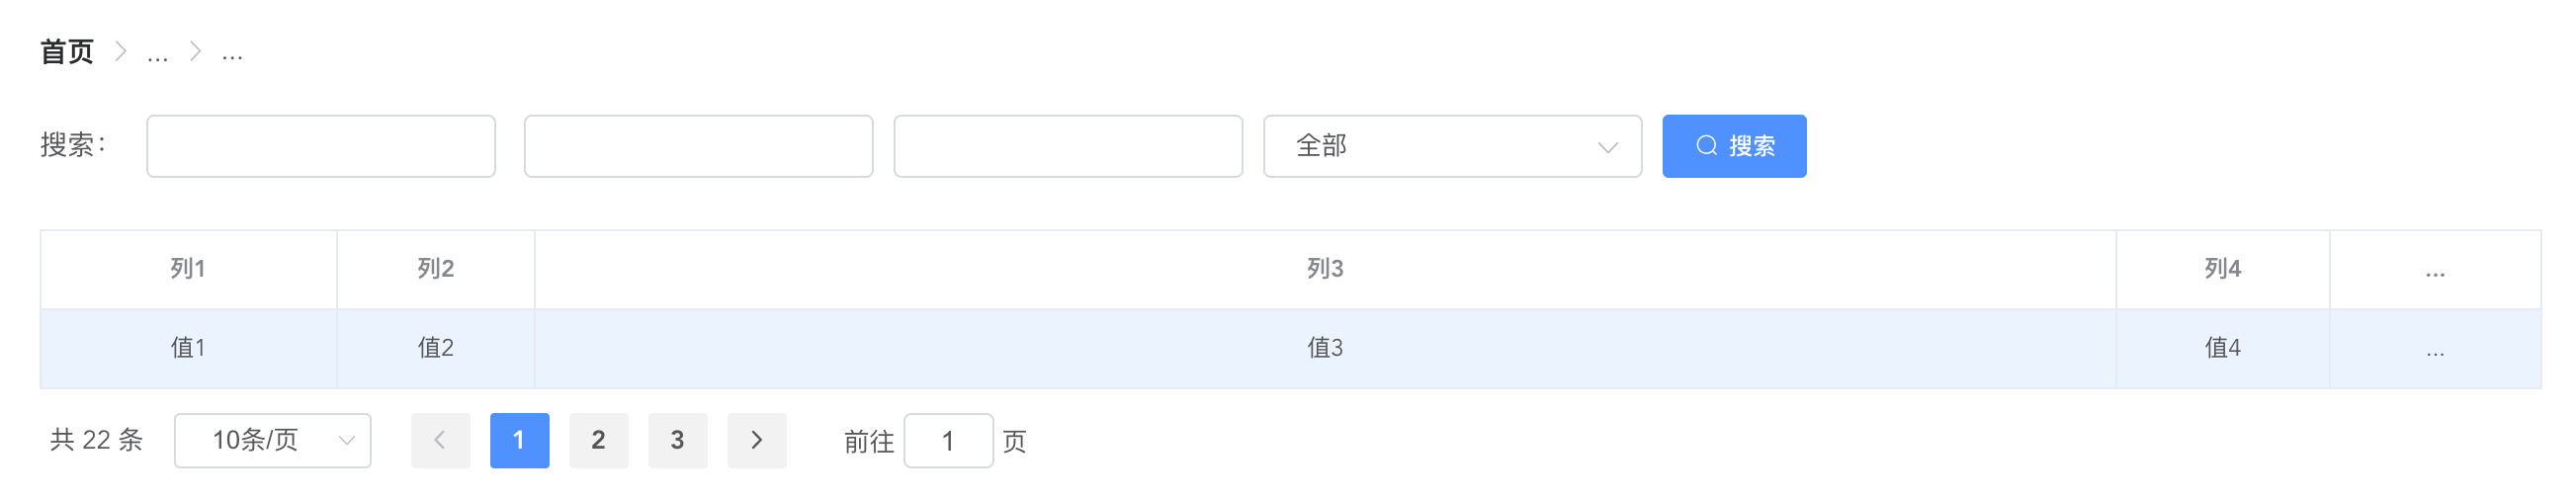
\includegraphics[width=1\linewidth]{./Figure/IMG_main.png}
    \caption{二级菜单页面结构}\label{Fig:main}
\end{figure}

\subsubsection{导航}
导航部分使用 Element-UI 的Breadcrumb 面包屑组件开发,可以现实从首页到当前页面的路径。
例如,当选择基础管理菜单下的二级菜单设备管理,这部分就会现实 “首页 > 设备管理”,如图 \ref{Fig:eg_main}。

\begin{figure}[ht]
    \centering
    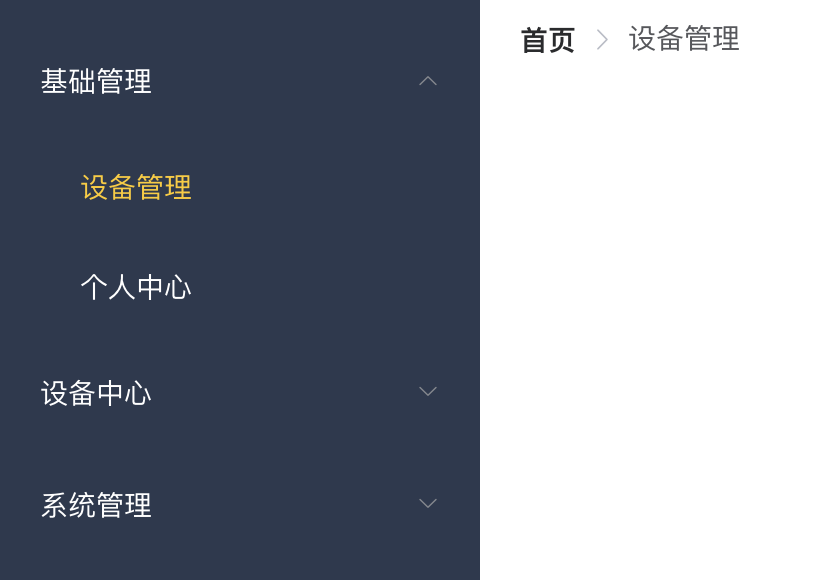
\includegraphics[width=0.6\linewidth]{./Figure/IMG_eg_main.png}
    \caption{一个导航实例}\label{Fig:eg_main}
\end{figure}

\subsubsection{搜索}
搜索栏用于对列表展示的内容进行搜索,可以通过指定搜索条件来展示不同的列表内容。
每一个二级菜单都有不同的搜索内容和选项。

例如在设备管理页面,搜索部分的内容如图 \ref{Fig:search_device} 所示,而在监控回放的页面,就如图 
\ref{Fig:search_replay} 所示。

\begin{figure}[ht]
    \centering
    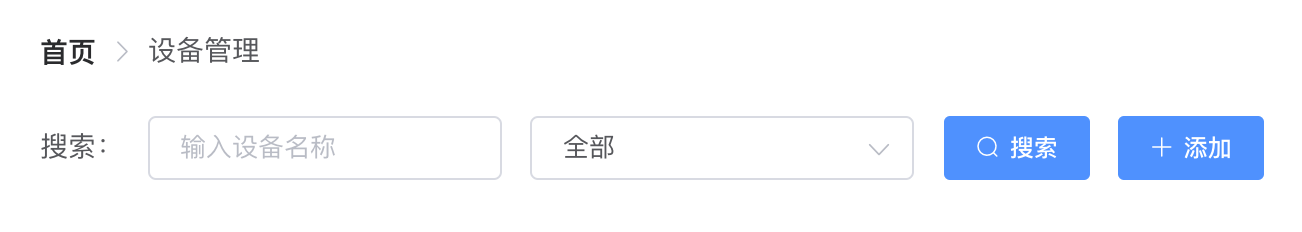
\includegraphics[width=0.9\linewidth]{./Figure/IMG_search_device.png}
    \caption{设备管理页面的搜索部分}\label{Fig:search_device}
\end{figure}

\begin{figure}[ht]
    \centering
    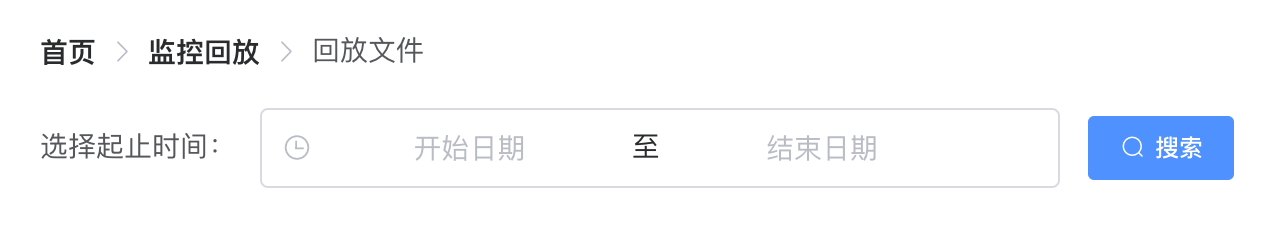
\includegraphics[width=0.9\linewidth]{./Figure/IMG_search_replay.png}
    \caption{监控回放页面的搜索部分}\label{Fig:search_replay}
\end{figure}

\subsubsection{列表}
列表页面展示数据,有后端接口返回。类似的,不同的页面列表部分展示的数据也不尽相同。
该部分展示的内容会受到搜索部分和分页部分影响。

\subsubsection{分页}
当数据过多时,后端会采用分页的方式返回数据,这一部分就是为了配合后端实现分页功能。
用户可以通过这个部分更改列表展示的数据条数和数据页数。

\newpage
\section{后端服务实现}
本节将介绍后端服务的实现,主要采用Spring Boot 框架开发,通过RESTful形式的HTTP 接口与前端交互。
\subsection{图形验证码接口}
图形验证码的作用是过滤无效的请求非认为请求,防止爬虫。
图形验证码接口时序图如图 \ref{Fig:code_seq} 所示。

\begin{figure}[ht]
    \centering
    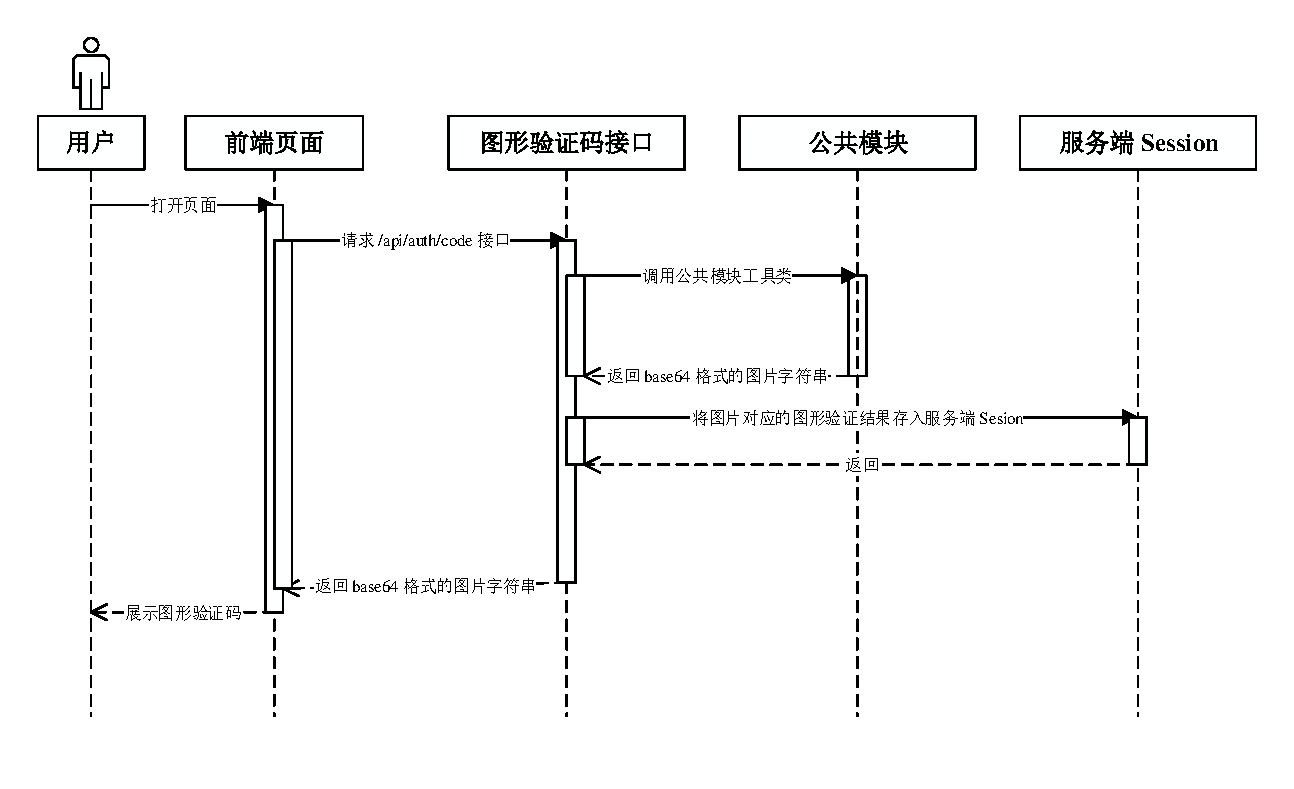
\includegraphics[width=1\linewidth]{./Figure/IMG_code_seq.pdf}
    \caption{图形验证码接口时序图}\label{Fig:code_seq}
\end{figure}

当用户打开本系统时,如果没有登陆过,则会跳转到登陆页面,之后就会请求图形验证码接口 /api/auth/code。
接口内部会调用公共模块的 VerifyUtil 类中的相关方法生产图形验证码,并返回二进制图片,Base64 编码格式的图片字符串和图形验证码。
图形验证码接口拿到公共模块的返回值后,会将图形验证码存入Session,并将 Base64编码格式的图形验证码返回给前端界面,最后前端
展示图片,如图 \ref{Fig:code_eg} 所示。

\begin{figure}[ht]
    \centering
    
\includegraphics[width=0.5\linewidth]{./Figure/IMG_code.png}
    \caption{图形验证码}\label{Fig:code_eg}
\end{figure}

\subsection{登陆接口}
用户在登陆页面输入用户名、密码和图形验证码,点击登陆按钮之后会调用后端接口。
接口地址为 /api/auth/login,接受的请求方法为POST,
需要三个参数:username(用户名)、password(密码)和 code(图形验证码)。后端再对这着三个参数进行
校验,如果通过则将用户信息和token(唯一标识符)返回。完整的时序图如 \ref{Fig:login_seq} 所示。

\begin{figure}[ht]
    \centering
    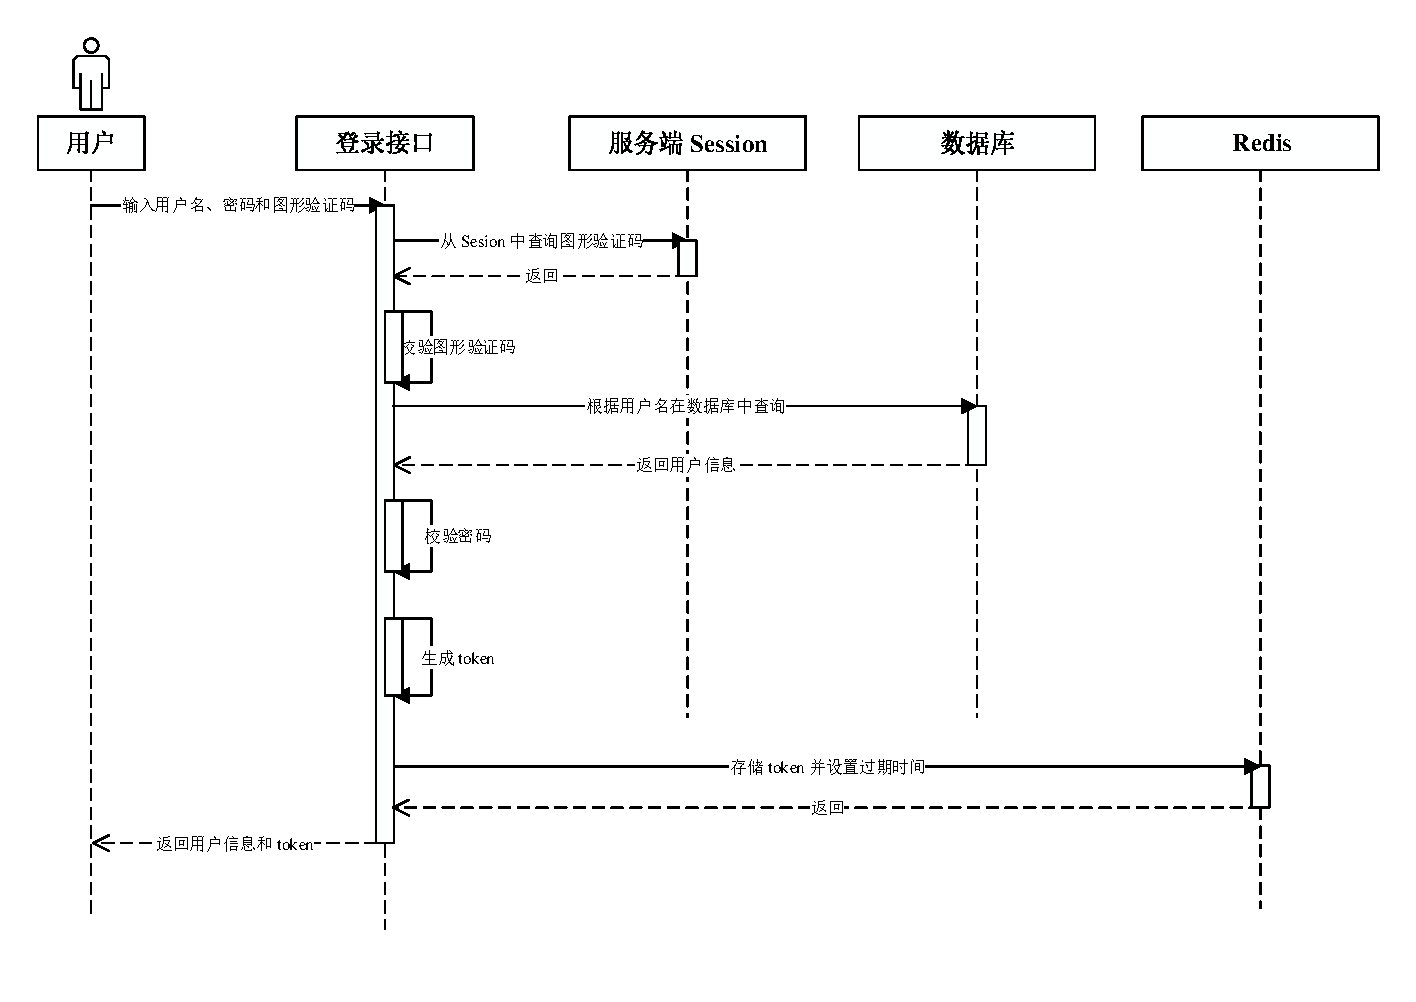
\includegraphics[width=1\linewidth]{./Figure/IMG_login_seq.pdf}
    \caption{登陆接口时序图}\label{Fig:login_seq}
\end{figure}

\subsection{列表查询接口}
列表页接口采用分页查询实现。
由于Mybatis-generator自动生成的Mapper并不支持分页查询的功能,因此通过使用扩展插件的方法,在
生成的代码中增加分页参数 limit 和 offset。
该接口与前端的分页组件联合使用,可以实现分页查询列表的功能。

此接口的实现并不复杂,因此不再赘述。

% \subsection{监控文件回放接口设计与实现}
% \subsubsection{视频录制}
\subsection{监控视频保存}
实时视频监控是通过在前端使用 flv.js 组件播放设备的 HTTP-FLV 直播流实现的。
本系统通过使用Java-CV依赖对设备的HTTP-FLV 直播流进行抓流并保存为MP4文件来实现监控视频的保存。

其中每一段视频的长度定为1分钟,同时为了使用户更方便的查找视频文件,
每一个视频的命名格式为“yyyy-dd-MM-HH-mm-ss.mp4”,并记录每个视频文件的录制开始时间和结束时间。
本系统通过定时任务,每隔一分钟遍历全部的摄像头,为每个摄像头创建一个一分钟的录制任务,并通过线程池来执行。
此外,在摄像头设备被添加到系统中时,也会同步启动一次视频录制。

监控视频保存的流程图如图 \ref{Fig:video_save} 所示。

\begin{figure}[ht]
    \centering
    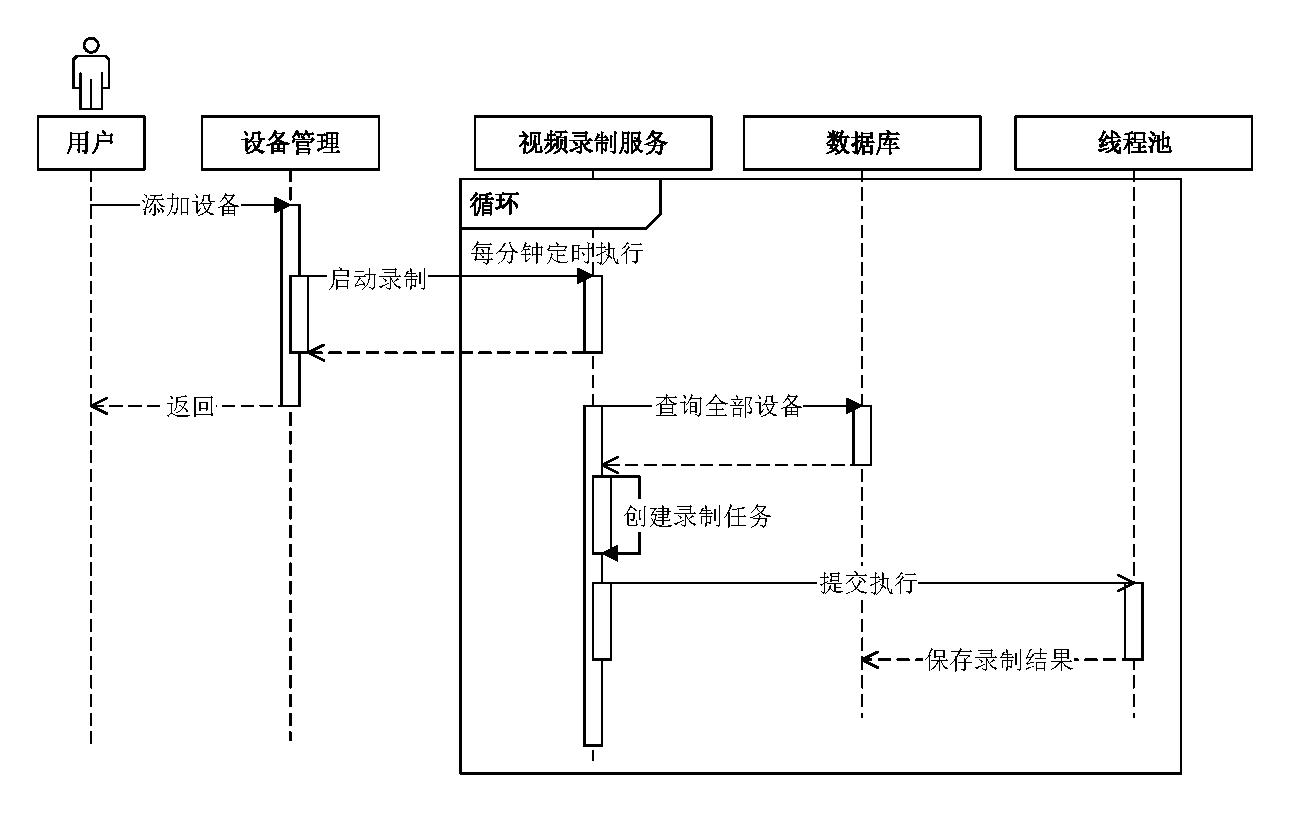
\includegraphics[width=1\linewidth]{./Figure/IMG_video_save.pdf}
    \caption{监控视频保存流程图}\label{Fig:video_save}
\end{figure}

\subsection{文件上传下载}
\subsubsection{文件上传}
文件上传接口用于个人中心修改头像功能。
% 如图 \ref{Fig:file_upload} 所示。
该接口利用Spring Boot 的 MultipartFile 实现,接口地址为/api/file/upload。
MultipartFile的内容是文件的二进制数据和文件名。在接口收到数据之后,可以通过 
MultipartFile 获取到文件的二进制数据和文件名,之后调用Java访问文件系统的相关方法,
将该文件保存在本地的文件系统中。最终返回一个文件的下载地址。

% http://<host>:<port>/api/file/download?filename=\$\{filename\}

% \newpage
% \begin{figure}[ht]
%     \centering
%     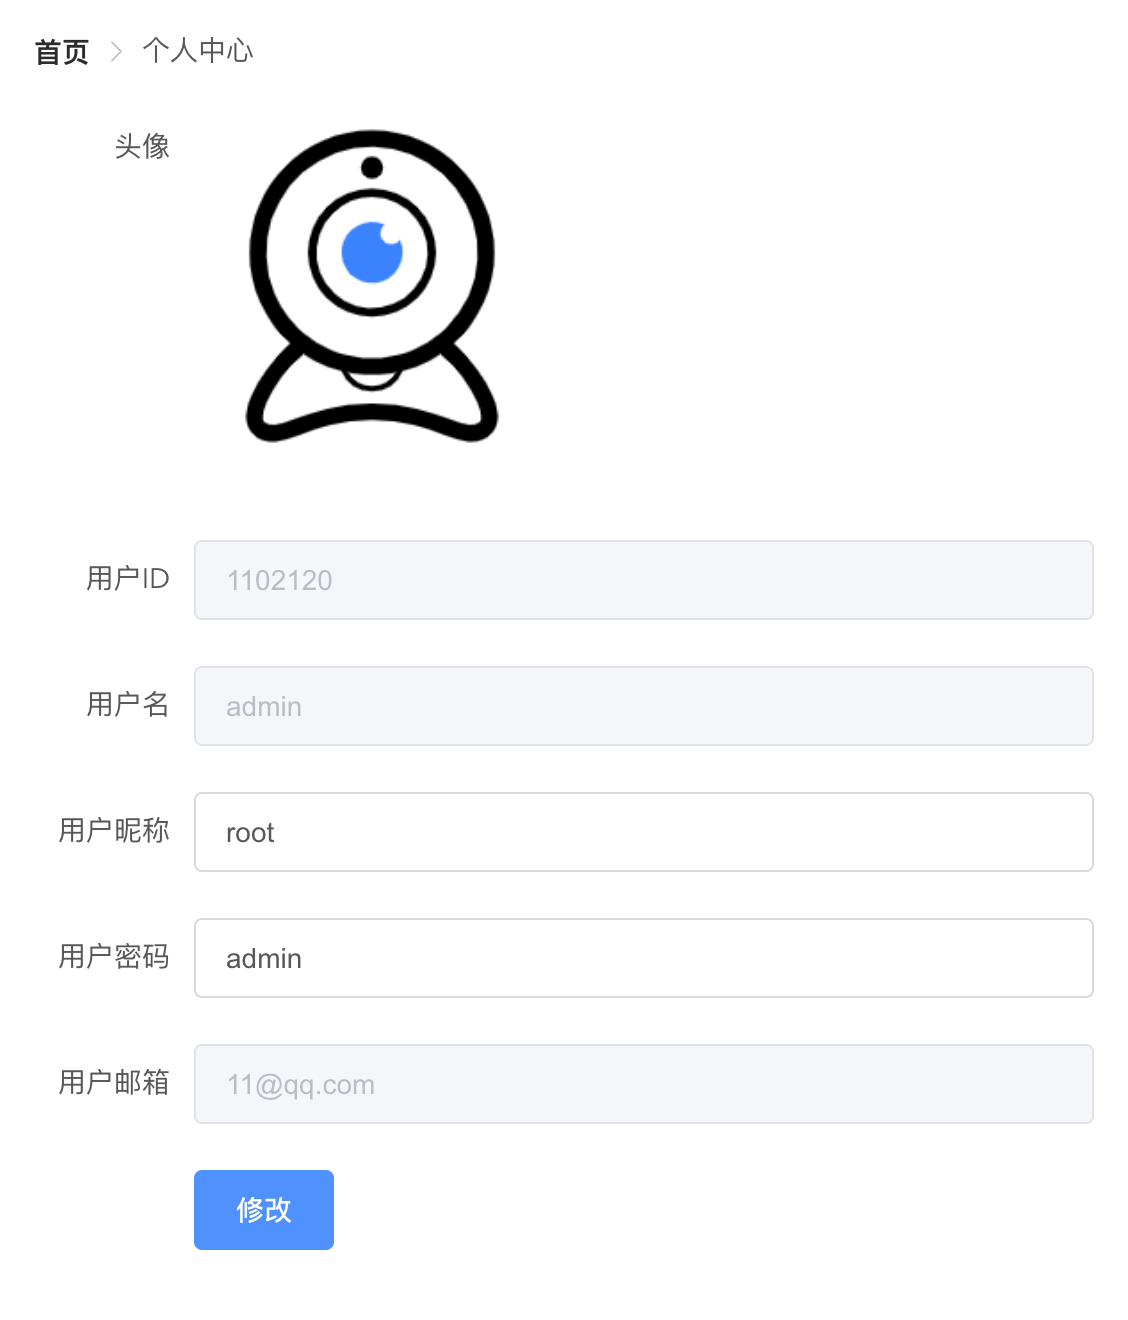
\includegraphics[width=0.5\linewidth]{./Figure/IMG_file_upload.png}
%     \caption{个人中心修改头像}\label{Fig:file_upload}
% \end{figure}
具体的流程图如图 \ref{Fig:seq_upload} 所示。

\begin{figure}[ht]
    \centering
    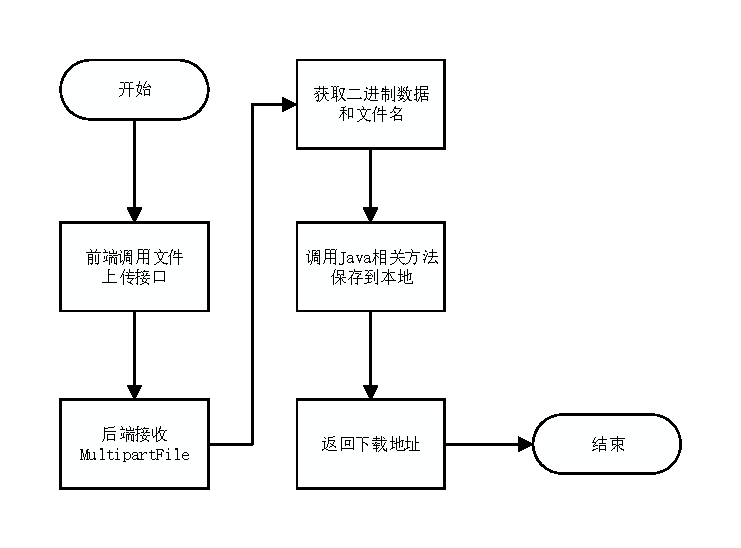
\includegraphics[width=1\linewidth]{./Figure/IMG_seq_upload.pdf}
    \caption{文件上传流程图}\label{Fig:seq_upload}
\end{figure}

\newpage
\subsubsection{文件下载}
文件下载接口用于个人头像的现实和视频监控回放文件的播放和下载功能中。
其接口实现较为简单,首先前端根据参数传递需要下载的文件的文件名,后端
通过Java访问文件系统打开对应文件获取到二进制的文件数据,
然后将其写入HttpServletResponse中,并设置 HTTP 返回值的Content-Type、
Character-Encoding,添加Content-Disposition的响应头。

具体的流程图如图 \ref{Fig:seq_download} 所示。

\begin{figure}[ht]
    \centering
    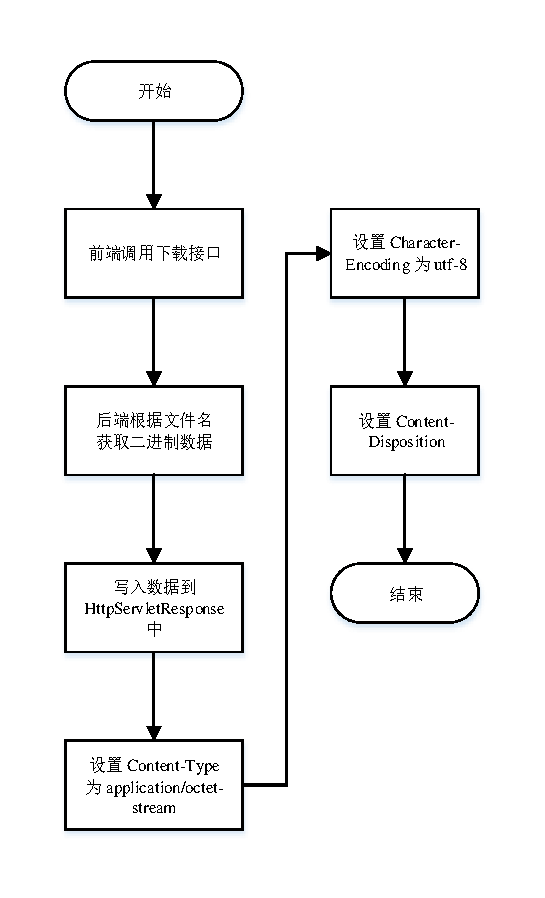
\includegraphics[width=1\linewidth]{./Figure/IMG_seq_download.pdf}
    \caption{文件下载流程图}\label{Fig:seq_download}
\end{figure}

\newpage
\section{系统测试}
本节的主要工作是对系统进行完成的测试,目的是检验系统设计是否达到需求分析的目标,各个功能是否正常使用。


% \newpage

% \chapter{系统测试}
% 本章的主要任务是对系统进行完成的测试,目的是检验系统设计是否达到需求分析的目标,各个功能是否正常使用。

\subsection{测试环境}
本系统有摄像头、服务端和客户端三部分组成。

摄像头采用奥尼生产的USB摄像头,分辨率为 1080P,如表 \ref{Tab:cam} 所示。
\begin{longtable}[ht]{|l|l|}
    \caption{测试摄像头配置表}
    \label{Tab:cam}\\
    % \begin{tabular}
    \hline
    品牌&奥尼\\
    \hline
    分辨率&1920*1080\\
    \hline
    最大帧率&30 FPS\\
    % \hline
    % 简要说明&用例变好\\
    \hline
    编码格式&MJPG \\
    \hline
    适应接口&USB2.0\\
    \hline
    \end{longtable}

服务端和客户端部署在同一台设备上,设备的配置如表 \ref{Tab:conf} 所示。

\begin{longtable}[ht]{|l|l|}
\caption{测试服务器配置表}
\label{Tab:conf}\\
\hline
操作系统&Windows 10\\
\hline
处理器&Intel Core i5-7400\\
\hline
内存&8G\\
% \hline
% 简要说明&用例变好\\
\hline
Redis&6.2.1 \\
\hline
MySQL&8.0.13\\
\hline
\end{longtable}

\newpage
\subsection{测试用例及结果}
测试方式采用黑盒测试,用于检验系统的功能是否正常。本节只介绍了关键功能的测试结果。

% \subsubsection{登陆功能测试}
% 用户首次打开系统时,会进入登陆页面,要求输入用户名、密码和图形验证码。
% 对于三个输入参数,只要存在一个不匹配,就会提示错误信息。表 \ref{Tab:login} 列出了部分测试用例以及测试结果。

% \begin{longtable}[ht]{|l|l|l|l|l|}
%     \caption{登陆功能测试用例以及结果}
%     \label{Tab:t_login}\\
%     \hline
%     序号&用例描述&测试输入&预期结果&结果\\
%     \hline
%     1&界面测试&1. 打开页面&1. 页面正常展示&通过\\
%     \hline
%     \multirow{4}*{2}&\multirow{4}*{正常登陆}&1. 输入正确的用户名密码&&\multirow{4}*{通过}\\
%     &&2. 输入正确的密码&提示登陆成功&\\
%     &&3. 输入正确的图形验证码&并跳转到首页&\\
%     &&4. 点击登陆按钮&&\\
%     \hline
%     \multirow{2}*{3}&\multirow{2}*{用户名异常}&1. 不输入用户名&提示用户名&\multirow{2}*{通过}\\
%     &&2. 输入不存在的用户名&或密码错误&\\
%     \hline
%     \multirow{2}*{4}&\multirow{2}*{密码异常}&1. 不输入密码&提示用户名&\multirow{2}*{通过}\\
%     &&2. 输入错误的密码&或密码错误&\\
%     \hline
%     \multirow{2}*{5}&\multirow{2}*{验证码错误}&1. 不输入验证码&\multirow{2}*{提示验证码错误}&\multirow{2}*{通过}\\
%     &&2. 输入错误的验证码&&\\
%     \hline
%     \multirow{4}*{6}&\multirow{4}*{记住密码}&1. 输入正确的用户名、密码&&\multirow{4}*{通过}\\
%     &&2. 输入正确的图形验证码&自动填充用户名&\\
%     &&3. 勾选记住密码&和密码&\\
%     &&4. 登陆后退出&&\\
%     \hline
% \end{longtable}


\subsubsection{实时监控功能测试}
用户可以在 “设备中心 > 实时监控 ”菜单下查看实时监控视频。
对于已经被删除的设备,不支持实时监控查看。
支持按照设备名称模糊搜索和按照设备类型精确搜索。
表 \ref{Tab:live_test} 列出了部分测试用例以及测试结果。

\begin{longtable}[ht]{|l|l|l|l|l|}
    \caption{实时监控功能测试用例以及结果}
    \label{Tab:live_test}\\
    \hline
    序号&用例描述&测试输入&预期结果&结果\\
    \hline
    1&界面测试&1. 打开页面&页面正常展示&通过\\
    \hline
    \multirow{2}*{2}&设备名称&1. 不输入设备名称&列表展示符合&\multirow{2}*{通过}\\
    &搜索&2.输入设备名称&条件的结果&\\
    \hline
    \multirow{2}*{3}&设备类型&1. 选择全部&列表展示符合&\multirow{2}*{通过}\\
    &搜索&2.选择除全部外的选项&条件的结果&\\

    \hline
    \multirow{2}*{4}&实时监控&\multirow{2}*{1. 点击查看实时监控视频按钮}&播放实时监控&\multirow{2}*{通过}\\
    &播放&&&\\

\hline
\end{longtable}


\newpage
\subsubsection{视频保存和检索功能测试}

用户可以在 “设备中心 > 监控回放 > 回放文件”菜单下查看实时历史的监控视频。
对于已经被删除的设备,同样也支持查看历史的监控视频。
用户可以在列表也下选中文件直接进行播放或者下载。
支持按照视频的起止时间进行范围搜索。
表 \ref{Tab:replay_test} 列出了部分测试用例以及测试结果。

\begin{longtable}[ht]{|l|l|l|l|l|}
    \caption{视频保存和检索测试用例以及结果}
    \label{Tab:replay_test}\\
    \hline
    序号&用例描述&测试输入&预期结果&结果\\
    \hline
    1&界面测试&1. 打开页面&页面正常展示&通过\\
    \hline
    \multirow{2}*{2}&\multirow{2}*{搜索}&1. 选择开始和结束时间&列表展示符合&\multirow{2}*{通过}\\
    &&2.不选择开始和结束时间&条件的结果&\\
    \hline
    3&播放文件&1. 点击播放按钮&文件开始播放&通过\\
    \hline
    4&下载文件&1. 点击下载按钮&文件开始下载&通过\\

\hline
\end{longtable}

\newpage
\subsubsection{设备列表功能测试}
用户可以在设备列表中进行以下操作:
\begin{enumerate}
    \item 根据设备名称进行模糊搜索
    \item 根据设备类型进行精确搜索
    \item 添加设备
    \item 修改设备信息
    \item 更改设备删除状态
\end{enumerate}

表 \ref{Tab:device_test} 列出了部分测试用例以及测试结果。

\begin{longtable}[ht]{|l|l|l|l|l|}
    \caption{设备列表功能测试用例以及结果}
    \label{Tab:device_test}\\
    \hline
    序号&用例描述&测试输入&预期结果&结果\\
    \hline
    1&界面测试&1. 打开页面&页面正常展示&通过\\
    \hline
    \multirow{2}*{2}&设备名称&1. 不输入设备名称&列表展示符合&\multirow{2}*{通过}\\
    &搜索&2.输入设备名称&条件的结果&\\
    \hline
    \multirow{2}*{3}&设备类型&1. 选择全部&列表展示符合&\multirow{2}*{通过}\\
    &搜索&2.选择除全部外的选项&条件的结果&\\
    \hline
    \multirow{4}*{4}&\multirow{4}*{添加设备}&1. 输入设备名称&\multirow{4}*{提示添加成功}&\multirow{4}*{通过}\\
    &&2. 选择设备类型&&\\
    &&3. 输入设备地址&&\\ 
    \hline
    \multirow{4}*{5}&\multirow{4}*{修改设备}&1. 修改设备名称&\multirow{4}*{提示修改成功}&\multirow{4}*{通过}\\
    &&2. 修改设备类型&&\\
    &&3. 修改设备地址&&\\
    &&4. 点击保存按钮&&\\
    \hline
    \multirow{2}*{6}&修改删除&1. 修改为删除&\multirow{2}*{设备删除状态变更}&\multirow{2}*{通过}\\
    &状态&2.修改为不删除&&\\
\hline
\end{longtable}




\section{本章小结}
本章分别从前端页面和后端服务两个角度对系统关键功能的实现进行了介绍。
之后介绍了系统关键功能的测试过程和结果,首先说明了系统的测试环境,然后陈述了系统关键功能的测试用例和结果。


\chapter{总结与展望}
\section{总结}
本文介绍了一种基于Spring Boot的视频实时监控系统的设计思路和实现方法。实现了如下功能:
\begin{enumerate}
    \item 链接安防摄像头,实时查看视频监控
    \item 视频按时间顺序保存并支持检索
    \item 用户登陆和权限管理
\end{enumerate}

本系统将传统的安防摄像头与互联网结合,使用户可以通过网页查看实时监控视频和历史视频监控,符合互联网时代的需求和发展潮流。

\section{展望}
本系统实现了实时监控视频查看、监控视频回放查看、监控视频回放检索等功能,但还是有很多可以完善和改进的地方。
首先,从功能方面,可以增加对监控摄像头操作移动的功能,现在市面上许多摄像头以及支持远程操作,只需要基于对方厂商提供的SDK进行二次开发即可。
其次,从性能方面,可以对监控视频的录制做改进,本系统是通过遍历全部的摄像头来发起视频录制任务,
但是对于自身带有存储的摄像头,可以直接通过厂商的SDK访问它的本地系统来进行回放文件的读取,无需再遍历。

\section{本章小结}
本章对本文完成的工作进行了总结和归纳,并对监控系统的设计和实现提出了自己的思考。